% -*- Mode:TeX -*-

%% IMPORTANT: The official thesis specifications are available at:
%%            http://libraries.mit.edu/archives/thesis-specs/
%%
%%            Please verify your thesis' formatting and copyright
%%            assignment before submission.  If you notice any
%%            discrepancies between these templates and the 
%%            MIT Libraries' specs, please let us know
%%            by e-mailing thesis@mit.edu

%% The documentclass options along with the pagestyle can be used to generate
%% a technical report, a draft copy, or a regular thesis.  You may need to
%% re-specify the pagestyle after you \include  cover.tex.  For more
%% information, see the first few lines of mitthesis.cls. 

%\documentclass[12pt,vi,twoside]{mitthesis}
%%
%%  If you want your thesis copyright to you instead of MIT, use the
%%  ``vi'' option, as above.
%%
%\documentclass[12pt,twoside,leftblank]{mitthesis}
%%
%% If you want blank pages before new chapters to be labelled ``This
%% Page Intentionally Left Blank'', use the ``leftblank'' option, as
%% above. 

\documentclass[12pt,twoside]{mitthesis}
\usepackage{lgrind}
%% These have been added at the request of the MIT Libraries, because
%% some PDF conversions mess up the ligatures.  -LB, 1/22/2014
\usepackage{cmap}
\usepackage[T1]{fontenc}
\pagestyle{plain}
\usepackage{graphicx}
\usepackage{amssymb}
\usepackage{amsmath}
\usepackage{calc}
\usepackage{supertabular}
\usepackage{subfigmat}
\usepackage{array}
\usepackage{textcomp}
\usepackage{listings}
\usepackage{hyperref}
\usepackage[acronym]{glossaries}
\makeglossaries

%% Create hyperlinks
\usepackage{hyperref}
\hypersetup{
    colorlinks,
    citecolor=black,
    filecolor=black,
    linkcolor=black,
    urlcolor=black
}
%%

\graphicspath{ {./figs/} }

\newcommand{\AR}{A\hspace{-2.0pt}R}
\newcommand{\TSFC}{{\rm T\!S\!F\!C}}
\newcommand{\RC}{{\rm R\!C}}

\newacronym{CE}{CE}{Convex Engineering}
\newacronym{CEG}{CEG}{Convex Engineering Group}
\newacronym{GP}{GP}{Geometric Programming}
\newacronym{gp}{GP}{Geometric Program}
\newacronym{SP}{SP}{Signomial Programming}
\newacronym{sp}{SP}{Signomial Program}
\newacronym{mdo}{MDO}{Multidisciplinary Design Optimization}
\newacronym{NLP}{NLP}{Nonlinear Programming}

% DISPLAYING PYTHON CODE
% Default fixed font does not support bold face
\DeclareFixedFont{\ttb}{T1}{txtt}{bx}{n}{12} % for bold
\DeclareFixedFont{\ttm}{T1}{txtt}{m}{n}{12}  % for normal

% Custom colors
\usepackage{color}
\definecolor{deepblue}{rgb}{0,0,0.5}
\definecolor{deepred}{rgb}{0.6,0,0}
\definecolor{deepgreen}{rgb}{0,0.5,0}
% Python style for highlighting
\newcommand\pythonstyle{\lstset{
language=Python,
basicstyle=\ttm,
otherkeywords={self},             % Add keywords here
keywordstyle=\ttb\color{deepblue},
emph={MyClass,__init__},          % Custom highlighting
emphstyle=\ttb\color{deepred},    % Custom highlighting style
stringstyle=\color{deepgreen},
frame=tb,                         % Any extra options here
showstringspaces=false            % 
}}


% Python environment
\lstnewenvironment{python}[1][]
{
\pythonstyle
\lstset{#1}
}
{}

% Python for external files
\newcommand\pythonexternal[2][]{{
\pythonstyle
\lstinputlisting[#1]{#2}}}

% Python for inline
\newcommand\pythoninline[1]{{\pythonstyle\lstinline!#1!}}

\begin{document}

%% -*-latex-*-
% 
% For questions, comments, concerns or complaints:
% thesis@mit.edu
% 
%
% $Log: cover.tex,v $
% Revision 1.8  2008/05/13 15:02:15  jdreed
% Degree month is June, not May.  Added note about prevdegrees.
% Arthur Smith's title updated
%
% Revision 1.7  2001/02/08 18:53:16  boojum
% changed some \newpages to \cleardoublepages
%
% Revision 1.6  1999/10/21 14:49:31  boojum
% changed comment referring to documentstyle
%
% Revision 1.5  1999/10/21 14:39:04  boojum
% *** empty log message ***
%
% Revision 1.4  1997/04/18  17:54:10  othomas
% added page numbers on abstract and cover, and made 1 abstract
% page the default rather than 2.  (anne hunter tells me this
% is the new institute standard.)
%
% Revision 1.4  1997/04/18  17:54:10  othomas
% added page numbers on abstract and cover, and made 1 abstract
% page the default rather than 2.  (anne hunter tells me this
% is the new institute standard.)
%
% Revision 1.3  93/05/17  17:06:29  starflt
% Added acknowledgements section (suggested by tompalka)
% 
% Revision 1.2  92/04/22  13:13:13  epeisach
% Fixes for 1991 course 6 requirements
% Phrase "and to grant others the right to do so" has been added to 
% permission clause
% Second copy of abstract is not counted as separate pages so numbering works
% out
% 
% Revision 1.1  92/04/22  13:08:20  epeisach

% NOTE:
% These templates make an effort to conform to the MIT Thesis specifications,
% however the specifications can change.  We recommend that you verify the
% layout of your title page with your thesis advisor and/or the MIT 
% Libraries before printing your final copy.
\title{Conceptual Engineering Design and Optimization Methodologies using Geometric Programming}


\author{Berk \"Ozt\"urk}
% If you wish to list your previous degrees on the cover page, use the 
% previous degrees command:
%       \prevdegrees{A.A., Harvard University (1985)}
% You can use the \\ command to list multiple previous degrees
%       \prevdegrees{B.S., University of California (1978) \\
%                    S.M., Massachusetts Institute of Technology (1981)}
\prevdegrees{B.S., Massachusetts Institute of Technology, 2016}
\department{Department of Aeronautics and Astronautics}

% If the thesis is for two degrees simultaneously, list them both
% separated by \and like this:
% \degree{Doctor of Philosophy \and Master of Science}
\degree{Master of Science in Aeronautics and Astronautics}

% As of the 2007-08 academic year, valid degree months are September, 
% February, or June.  The default is June.
\degreemonth{February}
\degreeyear{2018}
\thesisdate{February 1st, 2018}

%% By default, the thesis will be copyrighted to MIT.  If you need to copyright
%% the thesis to yourself, just specify the `vi' documentclass option.  If for
%% some reason you want to exactly specify the copyright notice text, you can
%% use the \copyrightnoticetext command.  
%\copyrightnoticetext{\copyright IBM, 1990.  Do not open till Xmas.}

% If there is more than one supervisor, use the \supervisor command
% once for each.
\supervisor{Mark Drela}{Professor, Aeronautics and Astronautics}

% This is the department committee chairman, not the thesis committee
% chairman.  You should replace this with your Department's Committee
% Chairman.
\chairman{Hamsa Balakrishnan}{Associate Professor, Aeronautics and Astronautics\\
Chair, Graduate Program Committee}

% Make the titlepage based on the above information.  If you need
% something special and can't use the standard form, you can specify
% the exact text of the titlepage yourself.  Put it in a titlepage
% environment and leave blank lines where you want vertical space.
% The spaces will be adjusted to fill the entire page.  The dotted
% lines for the signatures are made with the \signature command.
\maketitle

% The abstractpage environment sets up everything on the page except
% the text itself.  The title and other header material are put at the
% top of the page, and the supervisors are listed at the bottom.  A
% new page is begun both before and after.  Of course, an abstract may
% be more than one page itself.  If you need more control over the
% format of the page, you can use the abstract environment, which puts
% the word "Abstract" at the beginning and single spaces its text.

%% You can either \input (*not* \include) your abstract file, or you can put
%% the text of the abstract directly between the \begin{abstractpage} and
%% \end{abstractpage} commands.

% First copy: start a new page, and save the page number.
\cleardoublepage
% Uncomment the next line if you do NOT want a page number on your
% abstract and acknowledgments pages.
% \pagestyle{empty}
\setcounter{savepage}{\thepage}
\begin{abstractpage}
% $Log: abstract.tex,v $
% Revision 1.1  93/05/14  14:56:25  starflt
% Initial revision
% 
% Revision 1.1  90/05/04  10:41:01  lwvanels
% Initial revision
% 
%
%% The text of your abstract and nothing else (other than comments) goes here.
%% It will be single-spaced and the rest of the text that is supposed to go on
%% the abstract page will be generated by the abstractpage environment.  This
%% file should be \input (not \include 'd) from cover.tex.


Geometric programs (GPs) and other forms of convex optimization have recently experienced
a resurgence due to the advent of polynomial-time solution algorithms and improvements in computing.
Observing the need for fast and stable methods for multidisciplinary
design optimization (MDO),
previous work has shown that geometric programming can be a powerful framework
for MDO by leveraging the mathematical guarantees
and speed of convex optimization. However there exists a variety of barriers to
the implementation of optimization in design.
In this work, we formalize why the formulation
of non-linear design problems as GPs facilitates design.
Using the principles of pressure and boundedness,
we demonstrate the intuitive transformation of core physical and
data-based relations into GP-compatible constraints by systematically formulating an aircraft
design GP. We motivate the difference-of-convex extensions of GPs called signomial programs (SPs)
in order to extend the scope and fidelity of the model.
We detail the features specific to GPkit, an object-oriented GP formulation framework, which
facilitate the modern engineering design process.
Using both performance and mission modeling paradigms, we demonstrate the ability to
model and design increasingly complex systems in GP, and extract maximal engineering intuition
using sensitivities and tradespace exploration methods.
Though the methods are applied to an aircraft design problem, they are general to
models with continuous, explicit constraints, and lower the barriers to implementing
optimization in design.


\end{abstractpage}

% Additional copy: start a new page, and reset the page number.  This way,
% the second copy of the abstract is not counted as separate pages.
% Uncomment the next 6 lines if you need two copies of the abstract
% page.
% \setcounter{page}{\thesavepage}
% \begin{abstractpage}
% % $Log: abstract.tex,v $
% Revision 1.1  93/05/14  14:56:25  starflt
% Initial revision
% 
% Revision 1.1  90/05/04  10:41:01  lwvanels
% Initial revision
% 
%
%% The text of your abstract and nothing else (other than comments) goes here.
%% It will be single-spaced and the rest of the text that is supposed to go on
%% the abstract page will be generated by the abstractpage environment.  This
%% file should be \input (not \include 'd) from cover.tex.


Geometric programs (GPs) and other forms of convex optimization have recently experienced
a resurgence due to the advent of polynomial-time solution algorithms and improvements in computing.
Observing the need for fast and stable methods for multidisciplinary
design optimization (MDO),
previous work has shown that geometric programming can be a powerful framework
for MDO by leveraging the mathematical guarantees
and speed of convex optimization. However there exists a variety of barriers to
the implementation of optimization in design.
In this work, we formalize why the formulation
of non-linear design problems as GPs facilitates design.
Using the principles of pressure and boundedness,
we demonstrate the intuitive transformation of core physical and
data-based relations into GP-compatible constraints by systematically formulating an aircraft
design GP. We motivate the difference-of-convex extensions of GPs called signomial programs (SPs)
in order to extend the scope and fidelity of the model.
We detail the features specific to GPkit, an object-oriented GP formulation framework, which
facilitate the modern engineering design process.
Using both performance and mission modeling paradigms, we demonstrate the ability to
model and design increasingly complex systems in GP, and extract maximal engineering intuition
using sensitivities and tradespace exploration methods.
Though the methods are applied to an aircraft design problem, they are general to
models with continuous, explicit constraints, and lower the barriers to implementing
optimization in design.


% \end{abstractpage}

\cleardoublepage

\section*{Acknowledgments}

Firstly, I would like to thank Professor Warren Hoburg for giving me
the opportunity to work on research that I believe has great potential.
He introduced me to geometric programming and welcomed me to the Hoburg Research Group
(now the Convex Engineering Group). Under his mentorship, I learned that the most interesting designs
are the ones we don't expect, and that challenging current engineering design methods and norms
is the most worthwhile objective of optimization.
So thank you for the opportunity to do just that.

I am grateful for the many friends I have in the Aerospace Computational Design
Lab (ACDL) who have lightened my work hours with their camaraderie. Of this group,
the Convex folks reserve a special place. I am lucky to collaborate with
such a talented and dedicated group of researchers, and I hope that we will continue
to redefine conceptual engineering design.

This thesis would not have been possible without the amazing work Ned Burnell does
as the lead developer of GPkit. He never ceases to amaze me with his creativity and energy.
The many debates we have had about design philosophy have inspired this thesis,
and I'm glad I've gotten the opportunity to extensively document many of the ideas
that were discussed.

I thank my co-advisors Professor Mark Drela and Bob Haimes, who have taken on the burden of advising
me in Woody's absence. Thank you for your guidance and wisdom, and pushing me to
finish this thesis.

I am indebted to cycling for keeping me fit and sane. Cycling has given me opportunities to
escape, even as I miss winter training camp to conclude this thesis.
MIT Cyclists have been an immutable source of joy in my life, and are near and dear
to my heart. Thanks for enabling me.

I would like to thank my long-time friend Johannes Norheim
for being a battle-scarred companion through 5 years of MIT. We have been challenged, and
our paths have converged and diverged many times, but our friendship has not wavered.
My partner Elise Newman has been a ray of sunshine in every weather,
and I am looking forward to our future adventures together.

My parents definitely deserve a mention because I wouldn't exist without them.
The longer I live, the more I understand that I am where I am because of the
sacrifices they have made.
Deniz, you have been my rock. It has been my privilege to be your brother and watch
you grow up, and will be my privilege to help you
through your struggles and celebrate your future successes.
I am confident you will be more than I have been.

%%%%%%%%%%%%%%%%%%%%%%%%%%%%%%%%%%%%%%%%%%%%%%%%%%%%%%%%%%%%%%%%%%%%%%
% -*-latex-*-

% Some departments (e.g. 5) require an additional signature page.  See
% signature.tex for more information and uncomment the following line if
% applicable.
% \include{signature}

%\include{contents}
\chapter{Introduction}

Modern engineering design, and particularly aerospace design, has come to rely
heavily on optimization. Time and time again, the importance of fast and
reliable MDO tools has been stressed in the literature. However most MDO tools
have the downfalls of being slow due to the multimodal nature of many
engineering design problems.
	
In the \gls{CEG}, we seek to improve the engineering design process by
leveraging the mathematical guarantees and speed of convex optimization. We develop
open-source, object-oriented software to help build \gls{GP}-compatible models and
interface with solvers. In much of our previous work
(\cite{gp_ac_design},\cite{SP_ac_design}, \cite{sp_engine}), we have demonstrated that
\gls{GP} is useful for optimization, but have yet to formalize why it
facilitates design.
 
The mathematical restrictions on the form of constraints remains the biggest
barrier in the implementation of convex programs in design. Firstly, this thesis
will aim to show that the form of the GP actually facilitates the design process
and engineering understanding, rather than impeding it, through the disciplined use
of inequalities to express constraints. Hence it will aim to
pass on some of the expertise we have developed in the \gls{CEG} building
\gls{GP}-compatible models from general non-linear physical models. 

Secondly, it will aim to showcase the extensibility of \gls{GP} that is superior 
to other optimization formulations. The formulation of the \gls{GP} as a 'bag of 
constraints' instead of a hierarchial set of relations confers advantages 
when trying to expand the fidelity and scope of models, especially in the 
conceptual design stage. 

Finally, this thesis will discuss the features specific to GPkit in facilitating
an engineering design process that is streamlined and collaborative, and is
compatible with modern engineering design methodologies. The modularity of the 
models allows for a component-based design approach that ensures that designs 
satisfy the requirements both at the sub-system and complete-system levels. 
Furthermore, GPkit allows feedback between design engineers and models
which allows targeted efforts by engineers to collaboratively improve models.

\section{Defining Design versus Optimization} \label{sec:DesVsOpt}

It is difficult to find rigorous definitions of design and optimization that
try to identify the similarities and differences between the terms. For us to be
able to understand why \gls{GP}s facilitate design, we have to determine what 
features of optimization create barriers to entry for its use in design. 

\subsection{What is design?}

In the context of this paper, I will define design as the following:
	To design is to conceive the form and function of something. 

In the engineering sense, we think about the form as the configuration. 
In the product development sense, the form has more of an esthetic quality. 

The function is the actual purpose of the things being designed. It is oftentimes 
the aspect of the design that we can quantify (i.e. the performance). 

An important aspect of design is that it is a process. 

The underlying conclusion is that, to an optimization engineer, the classical 
definition of design implies a class of feasibility problems, given a set
of functional requirements. 

\begin{itemize}
\item Ned's comment: Parametrization and physics. Hard to agree on a representation 
that we all agree on. 
\end{itemize}

\subsection{What is optimization?}

Optimization has a rigorous mathematical definition: To optimize is to select an 
element in a set of feasible solutions with the lowest desired objective
function value. 

It is also a process, which is sensitive to the elements contained within the set
(related to the form), and the choice of objective function (related to the 
function).

In many ways, optimization is a natural extension of design, because it allows 
for an explicit mathematical representation of the form and function.

\subsection{The fundamental differences}

To many engineers, design and optimization are one and the same. However, 

\begin{itemize}
\item Design is human-driven. Optimization is computational. 
\item Design is based on feasibility. Optimization is based on the mathematical 
guarantees of optimality. 
\item Design can be done in non-restrictive mathematical forms. Optimization is 
done in specific mathematical forms that take advantage of structure. 
\end{itemize}

\section{Unifying design and optimization using gls{GP}}

\gls{GP} has developed "in response to a need to solve problems in the actual 
world".~\cite{duffingp} Quote from Duffin, 1967, main inventor of GP.

(Each section in this part of the intro has a corresponding section in the body.
(Each will feature an example problem that I will run through as a
(demonstration.)

There are three primary reasons why...

\begin{enumerate}     \item \textit{Inequalities help engineering
understanding.}

The mathematical constraints of \gls{GP} force designers to have a proper grasp
of the fundamental tradeoffs and pressures in a design.

Inequalities make feasible sets explicit. ADD A DIAGRAM OF FEASIBLE SETS using
SimPleAC HERE.

Traditionally, physical relations are expressed as equalities. But there is an
almost-seamless transition from fundamental physics to GP-compatible
constraints. ENGINEERS LIKE +VE QUANTITIES. eg. downforce vs. negative lift.

And even if the tradeoffs are not clear, we can use signomial equalities to
enforce constraints.

    \item \textit{Models are extensible.}
    
Models can be made arbitrarily complex. The 'bag of constraints' form of the GP
means that there is no need to reformulate the optimization scheme as more
constraints are added. This makes incremental modeling improvements possible and
even preferable.

The traditional engineering design process is split into conceptual, preliminary
and critical design segments. GP modeling facilitates this process by allowing
ever-increasing levels of complexity.

Gradient based optimization methods for multimodal systems often involves
converge loops, which have to be reengineered when new constraints are
introduced. VS. adding constraints to a bag...

We can effectively use sensitivity information to determine which parts of the
model yield the greatest returns to improved modeling, so engineers can target
their efforts.

    \item \textit{Models are flexible and modular, and compatible with modern
    engineering design (similar to extensible?)}

(This is a feature of GPkit, and not GPs in general.) \gls{GP}s make it easy to
implement component-based modeling, and build models that are shared between
different design problems. Each component has associated sizing and performance
variables.

This is helped by the fact that underconstrained \gls{GP}s can solve reliably,
and the tightness of constraints can be monitored.

\end{enumerate}




\chapter{Engineering inequalities and intuition, from equalities}
\label{ch2:inequalities}

This section will demonstrate how the form of the \gls{GP} (monomial
equalities and posynomial inequalities) helps engineers gain intuition
about the way that each variable is pressured
by a given objective function. Please refer to Appendices~\ref{a:gpintro} and ~\ref{a:spintro}
for detailed descriptions of the forms of \gls{GP}s and \gls{SP}s respectively.
The intuition gained in turn helps formulate
constraints that can properly bound each variable in the model.
GPkit, \gls{CEG}'s \gls{GP} modeling framework,
facilitates process by providing feedback to designers about
the boundedness of a model.

A simple aircraft optimization problem named SimPleAC\footnote{S and P have been capitalized to designate that
the model will be a 'signomial program', and AC is an acronym for 'aircraft'.} will be derived and will serve as
a demonstration of the intuitive structure of geometric and signomial programs, and show
how we can introduce new constraints to bound the feasibility sets of models.

\section{Making feasibility sets and boundedness explicit}

Consider the simple design problem below, where we define a simple bilinear
monomial equality with respect to $x$ and $y$, and constrain the sum of the variables
to be less than 2:

\begin{equation*}
\begin{aligned}
& {\text{minimize}}
& & x \\
& \text{subject to}
& & x + y \leq 2,
    & & & xy = \frac{1}{2} \label{simple_moneq}
\end{aligned}
\end{equation*}

We can draw the feasibility set of the above problem in both linear and log space,
as shown in Figure~\ref{f:feas_moneq}. One expects that, given only two variables
related through an equality and bounded by inequalities, the feasibility space is
a finite line segment in log-space, and a finite exponential function in linear space.
The black dot in Figure~\ref{f:feas_moneq} is the global optimum of the feasibility set
($x = 1 - \frac{1}{\sqrt{2}}$, $y = 1 + \frac{1}{\sqrt{2}}$).

\begin{figure}
    \centering
    \includegraphics[width=0.8\textwidth]{feas_moneq.png}
    \caption{The $x$-$y$ feasibility set of a simple monomial equality.}
    \label{f:feas_moneq}
\end{figure}

However, if we had decided to impose $xy \geq \frac{1}{2}$ instead of $xy = \frac{1}{2}$,
then we would get a new feasibility set as shown in Figure~\ref{f:feas_posygeq}.
Using the \gls{GP} form, we can always upper-bound posynomials, and lower-bound both posynomials
and monomials to get convex feasible sets. Note that the optimal point, which is at
$x = 1 - \frac{1}{\sqrt{2}}$, $y = 1 + \frac{1}{\sqrt{2}}$,
does not change when the monomial equality is relaxed. This is a key
observation that will allow us to turn the equalities in most physical models into \gls{GP}-compatible
posynomial inequalities. The posynomial equality relaxation is explained in greater detail
in~\cite{hoburg_thesis}.

\begin{figure}
    \centering
    \includegraphics[width=0.8\textwidth]{feas_posygeq.png}
    \caption{The $x$-$y$ feasibility set of lower-bounding monomial,
    and upper-bounding posynomial.}
    \label{f:feas_posygeq}
\end{figure}

However if we convert the monomial equality to  $xy \leq \frac{1}{2}$, we will get an unbounded model,
whose feasibility set is shown in Figure~\ref{f:feas_posyleq}.
Since minimizing $x$ is our objective, and both variables are upper-bounded,
they both collapse towards numerical precision zero,
giving a vanishing feasibility set shown in Figure~\ref{f:feas_posyleq}. This section will
demonstrate methods to create \gls{GP}-compatible models that are adequately bounded to avoid such
singularities towards zero or infinity, which for the most part do not
exist in real physical models. The models will be created within GPkit~\cite{gpkit}.

\begin{figure}
    \centering
    \includegraphics[width=0.8\textwidth]{feas_posyleq.png}
    \caption{The $x$-$y$ feasibility set of upper-bounding monomial,
    and upper-bounding posynomial.}
    \label{f:feas_posyleq}
\end{figure}

\section{Defining the design problem}

\gls{GP}s are amenable to solving a large variety of design problems (see~\cite{gpintro} for an
extensive number of examples). This thesis uses aircraft design to demonstrate
design methodologies that leverage convex optimization since the author's background is in aerospace engineering.
Aircraft epitomize the nature of complex engineering problems. The physical 
relations describing their motion are nonlinear, and all of their subsystems are 
coupled through the primary forces in flight (thrust, weight, lift, drag).
The goal of the aircraft in question will be to perform a basic `ferry' mission, that
is to carry a given payload
over a distance while minimizing an objective function.

\subsection{Objective functions}
\label{s:objective}

Objective functions are the way that a designer puts pressure on the variables 
in the constraints. To begin with, we will consider
total fuel weight $W_f$ as our objective, which will put
downward pressure on all of the variables that would cause greater fuel burn, namely
drag and weight. We must necessarily lower-bound all variables in the objective function
that have positive exponents, and upper-bound all variables with negative exponents.

In many design problems
formulated as \gls{GP}s, many different objectives will put pressure on design
in the same direction. For example, an aircraft optimized for fuel weight will look
different compared to one
that has been designed for total weight or payload-fuel consumption, but each
of these objectives will put a downward pressure on drag and weight.
As such, this model will be able to take in a number of objective functions
and be properly constrained and bounded. According to Raymer, an important
principle of aircraft design is `that there is no such thing as a free lunch!'
~\cite[pg.26]{raymer}. An improvement in any of the other objective functions
will result in reduced performance with respect to others.

\subsection{Functional description: constraining the problem}

The typical process for designing anything usually involves doing either a
component decomposition or a functional decomposition of the problem. In
this case, we will think about the functional decomposition to create a
basic list of constraints that our aircraft will need to fulfill to be
able to capture the tradeoffs in an aircraft design problem. (In
Section~\ref{s:submodels}, we will examine how thinking about the component decomposition
can help structure larger problems.)

What does an aircraft need to be able to do to deliver payload of a distance?
\begin{itemize}
	\item It will need to sustain steady
    level flight, keeping itself and the payload aloft (Section~\ref{s:wl}).
    \item It will need to overcome drag (Section~\ref{s:td}).
	\item It will need to contain enough fuel to complete its mission
        (Section~\ref{s:fuel}).
	\item It will need to be able to sustain its structural loads (Section~\ref{s:wingstrc}).
\end{itemize}

Note that these are in no way presented in order of importance, which is reflective
of the non-hierarchical nature of \gls{GP}s.
In the basic example, we will choose not to model engines,
and leave this as an exercise
to complete in Section~\ref{s:engine} to improve the model.

\section{GP Modeling from Physics}

Optimization model creation often starts haphazardly, with the designer having a
vague idea about the set of physics that govern a problem, and some basic
assumptions about the configuration. In this section, we will
generate variables and constraints with abandon, and think about how to make
sure each variable is adequately bounded later. Each subsection is intended
to introduce the reader to an important aspect of \gls{GP} modeling,
accompanied by examples in implementation.

\subsection{Free and fixed variables: modeling weight and lift}
\label{s:wl}

For this particular design problem, we start by modeling
weight and lift, since one fundamental function of the aircraft is to stay aloft.
The aircraft has weight, which consists of the payload, wing, and fuel weights. 

\begin{equation}
    W \geq W_p + W_w + W_f
\end{equation}

Note that we have already had to make determination about the relation between
the two sides of the equation. Heavier aircraft burn more fuel, so we are justified
to put total weight as greater than the sum of the component weights since
$W$ will be pressured downward by the objective. Furthermore, we can
always add more weight to the aircraft by adding ballast to it, even if this would likely
worsen the objective. So we allow for slackness in this constraint, even
if we know intuitively that it will almost always be tight as explained in Section~\ref{s:objective}.

The aircraft has to sustain steady level flight, which means
that it needs to generate enough lift to carry itself. We use the naive
lift is greater than weight ($L \geq W$)
model below for steady state flight:

\begin{equation}
   \frac{1}{2} \rho V^2 S C_L  \geq  W_p + W_w + 0.5 W_f
\end{equation}

where the lift of the aircraft is equal to weight of the aircraft with half-fuel, 
which is a crude estimate of the average weight of the aircraft throughout the flight.
Again, the \gls{GP} form is seamless here, since lift is related to
induced drag, and so it is pressured downward into the posynomial on the \gls{RHS} of the equation.

We would also like the fully-fueled aircraft to be able to fly at a minimum speed 
of $V_{min}$ without stalling, so we add the following constraint:

\begin{equation}
    W \leq \frac{1}{2} \rho V_{min}^2 S C_{L_{max}}
\end{equation}

Note that, although we could use a monomial equality here, we don't, because this
relation does not need to be tight. It is acceptable that the aircraft is able to
fly at a velocity slower than $V_{min}$ for a given objective function.

At this point, we have introduced a large set of variables, some of which are input
parameters, and the others free variables. The decision of whether to keep variables free or fixed
can shape the whole model development process in all forms of optimization.
The decision can be influenced by many
factors in a \gls{GP}, with four in particular that stand out in this model.
We set the lift coefficient and takeoff speed
to be constants since (I) we would need
more detailed modeling to determine their values. Payload weight is set
because (II) it would always be unbounded towards zero due to the downward pressure from
the objective. A designer may also fix variables (III) if he/she knows their values with
certainty (e.g.\ gravitational acceleration $g$) or (IV) the variable is a normalizing
coefficient (which we will see in Section~\ref{s:datafit}).
The variables have been defined in Table~\ref{t:vars_WandL}, where the variables that
have associated values are fixed variables.
The remaining variables are free variables, to be optimized once the model
is appropriately bounded.

\begin{footnotesize}
\begin{table}
    \centering
    \begin{tabular}{ l c c l}
        \toprule
        \textbf{Variable} & \textbf{Value} & \textbf{Units} & \textbf{Description} \\
        \midrule
        $\rho$ & 1.23 & $~\mathrm{\tfrac{kg}{m^{3}}}$ & density of air \\
        $C_L$ & \ldots & $~\mathrm{-}$ & wing lift coefficient \\
        $C_{L,max}$ & 1.6 & $~\mathrm{-}$ & lift coefficient at stall \\
        $S$ & \ldots & $~\mathrm{m^{2}}$ & total wing area \\
        $V$ & \ldots & $~\mathrm{\tfrac{m}{s}}$ & cruising speed \\
        $V_{min}$ & 25 & $~\mathrm{\tfrac{m}{s}}$ & takeoff speed \\
        $W$ & \ldots & $~\mathrm{N}$ & total aircraft weight \\
        $W_f$ & \ldots & $~\mathrm{N}$ & fuel weight \\
        $W_w$ & \ldots & $~\mathrm{N}$ & wing weight \\
        $W_p$ & 6250 & $~\mathrm{N}$ & payload weight \\
        \bottomrule
    \end{tabular}
    \caption{Variables introduced in weight vs. lift model.}
    \label{t:vars_WandL}
\end{table} \end{footnotesize}

Note that the atmospheric variable $\rho$ in Table~\ref{t:vars_TandD}, and other
atmospheric variables in Section~\ref{ch2:inequalities} are set
to be constant. The behavior of these variables with altitude
will be modeled in more detail in Section~\ref{s:mission} when
the flight profile of the aircraft is modeled.

\subsection{Alternate objectives: adding performance metrics}
\label{s:altobj}

As multi-objective designers, we may also be interested in knowing about
additional performance metrics that can serve as part of objective functions. A
few that are particularly relevant to aircraft will be introduced here.

The time of flight of the aircraft, which is a useful metric to calculate cost,
is simply the aircraft's range divided by its cruise velocity:

\begin{equation}
    T_{flight} \geq \frac{\mathrm{Range}}{V}
\end{equation}

The lift-to-drag ratio is also defined: 

\begin{equation}
    L/D = \frac{C_L}{C_D}    
\end{equation}

The new variables we have introduced are detailed in Table~\ref{t:vars_perfMetrics}.

\begin{footnotesize}
\begin{table}
    \centering
    \begin{tabular}{ l c c l}
        \toprule
        \textbf{Variable} & \textbf{Value} & \textbf{Units} & \textbf{Description} \\
        \midrule
        $C_D$ & \ldots & $~\mathrm{-}$ & drag coefficient \\
        $C_L$ & \ldots & $~\mathrm{-}$ & wing lift coefficient \\
        $L/D$ & \ldots & $~\mathrm{-}$ & lift-to-drag ratio \\
        $Range$ & 3000 & $~\mathrm{km}$ & aircraft range \\
        $T_{flight}$ & \ldots & $~\mathrm{hr}$ & flight time \\
        \bottomrule
    \end{tabular}
    \caption{Variables introduced to define new performance metrics.}
    \label{t:vars_perfMetrics}
\end{table} \end{footnotesize}

An important note about variables that are potential alternate objectives: these variables
must always be lower-bounded (or inverted and upper-bounded) since the general \gls{GP} is a
minimization problem. However, if they are not also upper-bounded, these variables
will likely be unbounded for a given model and run off to +$\infty$. This means that
performance-quantifying variables will need to be in a monomial form,
or must be present in a posynomial objective
function as shown in Equation~\ref{e:posyobj} for boundedness. We shall see this coming into play
in Section~\ref{s:missionobj}.

\begin{equation}
    \mathrm{Objective} \geq \sum\limits^n_{i=1}c_{i}\prod\limits^n_{i=1}  v^{k_{i,j}}
    \label{e:posyobj}
\end{equation}

\subsection{More physics for boundedness: thrust and drag model}
\label{s:td}

If we attempt to run our current model, we would find that it is unbounded in many variables.
The results are shown in Table~\ref{t:WandL_unbounded}.

\begin{footnotesize}
\begin{table}
    \centering
    \begin{tabular}{ l c l }
        \toprule
        Unbounded variable & Units & Direction \\
        \midrule
        $S$ & $~\mathrm{m^{2}}$ & $\infty$ \\
        $T_{flight}$ & $~\mathrm{hr}$ & $\infty$ \\
        $V$ &  $~\mathrm{\tfrac{m}{s}}$  & $\infty$ \\
        $W_f$ & $~\mathrm{N}$ & $0$ \\
        $W_w$ & $~\mathrm{N}$  & $0$ \\
        \bottomrule
    \end{tabular}
    \caption{Unbounded variables in the weight and lift model.}
    \label{t:WandL_unbounded}
\end{table} \end{footnotesize}

This is not surprising at all, since none of the defined variables lower-bound $W_f$,
the objective function, in the constraints we have defined.
Without the pressure from the objective, any variables that
are not both upper- and lower- bounded will tend to blow up. This is indicative usually
that more modeling or direct substitutions are required to sufficiently bound the variables.

In this case, we lack a propulsion model which would properly bound fuel weight, velocity,
and time of flight. For initial modeling purposes, we assume a naive constant brake
specific fuel consumption (\BSFC) for the 'engine' of the aircraft, which is assumed
to provide as much thrust as needed. Since $T \geq D$:

\begin{equation}
    W_f \geq \BSFC \times T_{flight} \times DV
    \label{e:W_f}
\end{equation}

the fuel weight required is the product of the \BSFC, time of flight, and the
total drag power on the aircraft.
The drag of the aircraft is the product of dynamic pressure ($\frac{1}{2} \rho V^2$),
the planform area $S$, and the coefficient of drag of the aircraft:

\begin{equation}
    D \geq \frac{1}{2} \rho V^2 S C_D
    \label{e:d}
\end{equation}

There are yet more relaxed monomial equalities in Equations~\ref{e:W_f} and \ref{e:d}.
If the pressure on the \gls{LHS} or \gls{RHS} of a monomial equality are clear as in these cases,
it is a good practice to relax the equality to leave as many degrees of freedom
in the design space as possible. The intuition is that, we can almost always spend more fuel or have more drag,
but the constraints will always be tight since all objectives will suffer as a consequence.

The drag coefficient of the aircraft is assumed to be the sum of the fuselage drag,
the wing profile drag, and the wing induced drag coefficients \cite{gp_ac_design}:

\begin{equation}
    C_D \geq C_{D_{fuse}} + C_{D_{wpar}} + C_{D_{ind}}
\label{e:cd}
\end{equation}

The individual components of the drag are represented as monomial equalities, again borrowing
from \cite{gp_ac_design} for constraints~\ref{e:cdfuse} through~\ref{e:cdinduced}.
The fuselage drag is a function of its drag area $\CDA_0$ and the planform area of the wing:

\begin{equation}
    C_{D_{fuse}} = \frac{\CDA_0}{S}
\label{e:cdfuse}
\end{equation}

where the $\CDA_0$ is linearly proportional to the volume of fuel in the fuselage:

\begin{equation}
    V_{f_{fuse}} = \CDA_0 \times 10 ~\mathrm{[meters]}
\label{e:vffuse}
\end{equation}

Note that we correct the dimensionality of the volume here, since GPkit automatically checks units.

The wing profile drag is the product of the form factor, the friction drag coefficient,
and the wetted area ratio of the wing \cite{gp_ac_design},

\begin{equation}
    C_{D_{wpar}} = k C_f S_{wetratio}
\label{e:cdwpar}
\end{equation}

The Reynolds number of the aircraft wing is approximated

\begin{equation}
    Re \leq \frac{\rho}{\mu} V \sqrt{\frac{S}{\AR}}
\label{e:re}
\end{equation}

and used to find the friction drag coefficient of wing. We approximate the $C_f$ by assuming a
turbulent flat plate flow:

\begin{equation}
    C_f \geq \frac{0.074} {Re^{0.2}}
\end{equation}

The induced drag of the wing is calculated with a span efficiency factor $e$, and is a
function of the $C_L$ and aspect ratio \AR of the wing.

\begin{equation}
    C_{D_{induced}} = \frac{C_L^2}{\pi \AR e}
\label{e:cdinduced}
\end{equation}

The new variables are detailed in Table~\ref{t:vars_TandD}.

\begin{footnotesize}
\begin{table}
    \centering
    \begin{tabular}{ l c c l}
        \toprule
        \textbf{Variable} & \textbf{Value} & \textbf{Units} & \textbf{Description} \\
        \midrule
        \AR & \ldots & $-$ & aspect ratio\\
        $\BSFC$ & 400 & $\mathrm{\frac{g}{kW*hr}}$ & brake specific fuel consumption \\
        $\CDA_0$ & \ldots & $~\mathrm{m^{2}}$ & fuselage drag area \\
        $C_f$ & \ldots & $-$ & skin friction coefficient \\
        $D$ & \ldots & $~\mathrm{N}$ & total drag force \\
        $e$ & 0.92 & $-$ & Oswald efficiency factor \\
        $k$ & 1.17 & $-$ & form factor \\
        $\mu$ & $\mathrm{1.78 \times 10^{-5}}$ & $~\mathrm{\tfrac{kg}{m\cdot s}}$ & viscosity of air \\
        $Re$ & \ldots & $-$ & Reynolds number \\
        $\left(\frac{S}{S_{wet}}\right)$ & 2.075 & $-$ & wetted area ratio \\
        $V_{f_{fuse}}$ & $~\mathrm{m^{3}}$ & \ldots & fuel volume in the fuselage \\
        \bottomrule
    \end{tabular}
    \caption{Variables introduced in thrust and drag model.}
    \label{t:vars_TandD}
\end{table} \end{footnotesize}

%\begin{python}
%        # Thrust and drag model
%        C_D_fuse = CDA0 / S
%        C_D_wpar = k * C_f * S_wetratio
%        C_D_ind  = C_L ** 2 / (np.pi * A * e)
%        constraints += [W_f >= BSFC * T_flight * D,
%                    D >= 0.5 * rho * S * C_D * V ** 2,
%                    C_D >= C_D_fuse + C_D_wpar + C_D_ind,
%                    V_f_fuse == 10*units('m')*CDA0,
%                    Re <= (rho / mu) * V * (S / A) ** 0.5,
%                    C_f >= 0.074 / Re ** 0.2]
%\end{python}

As shown in Table~\ref{t:WLTD_unbounded}, attempting to run the model as is
results in both the fuselage fuel
volume $V_{f_{fuse}}$ and the wing weight $W_w$ still having no lower bounds.
These variables will need to be properly bounded to complete the SimPleAC model.

\begin{footnotesize}
    \begin{center}
        \begin{table}
            \begin{tabular}{ l c l }
                \toprule
                Unbounded variable & Units & Direction \\
                \midrule
                $V_{f_{fuse}}$ &  $~\mathrm{m^3}$  & $0$ \\
                $W_w$ & $~\mathrm{N}$  & $0$ \\
                \bottomrule
            \end{tabular}
            \caption{Unbounded variables within the GP formulation}
            \label{t:WLTD_unbounded}
        \end{table}
    \end{center}
\end{footnotesize}

\section{Limits of GP and Convexity, and SP modeling}
\label{s:GPlimits}

Even with the demonstrated strengths of \gls{GP}s in solving certain classes of
problems, it is important to recognize that the mathematical framework has limits.
The three distinct types of~\gls{GP}-incompatibility in design problems are detailed
by Hoburg~ \cite{hoburg_thesis}, which are discreteness,
quasi-convexity, and multi-modality. Discreteness in \gls{GP} can be approached
by coupling discrete programming methods such as branch-and-bound into a sequential
\gls{GP}. This is outside of the scope of this thesis.
Quasi-convexity and to a certain extent multimodality can
be addressed through a non-log-convex extension of \gls{GP}s called \gls{SP}s, where
certain constraints are expressed as signomial (or difference-of-posynomial) constraints
(described in greater detail in Appendix~\ref{a:spintro}).
Even the addition of a single
signomial constraint turns the problem from a \gls{GP} to a \gls{SP}, which means
that the problems loses convexity and all of the mathematical guarantees associated with it. 
It takes engineering intuition to recognize where and when improved modeling is worth
the loss of the mathematical guarantees. Kirschen~\cite{kirschen_thesis} describes in detail how
signomial constraints are often required to capture fundamental design tradeoffs.

\subsection{Signomial constraints: adding fuel volume model}
\label{s:fuel}

In an attempt to put a lower bound $V_{f_{fuse}}$, we will
be adding a fuel volume model to SimPleAC, where fuel can be stored in the wing or
in the fuselage. The fuel volume will be modeled first instead of the wing
weight because the wing weight will be a function of the fuel stored in the fuselage.
The reason why this model is \gls{GP}-incompatible is because of the
following constraint which follows logically:

\begin{equation}
	V_{f_{avail}} \leq V_{f_{wing}} + V_{f_{fuse}}
	\label{vfavail}
\end{equation}

The fuel volume available must be less than the sum of the fuel volume available in the
wing and the fuselage. It turns out that volumes that 'contain' free variables
can create signomial constraints. (One way around this is potentially creating fuel
fraction variables to denote how much fuel is stored in each volume, but
other potential parametrizations will not be explored here.)

As such, we can continue to develop the model, since it is important for us to
capture the fuel distribution between the wing and the fuselage. Fuel weight is going
to influence the lift required of the aircraft, so the weight of the fuel is determined
using a density parameter $\rho_{f}$. 

\begin{equation}
    V_f = \frac{W_f } {\rho_f g}
    \label{e:vf}
\end{equation}

We need a model of how much fuel volume there is in a wing. Intuitively,
we would expect the volume within a wing
to be related linearly to its thickness ratio ($\tau$) and span ($b$),
and to the square of its chord ($c$). 

\begin{equation}
	V_{f_{wing}} \propto \tau b c^2
	\label{e:vfwingpre}
\end{equation} 

It is convenient to express relation~\ref{e:vfwingpre} in terms of planform area $S$,
aspect ratio \AR~and thickness ratio $\tau$ only.
Using the additional relations $\AR = \frac{b^2}{S}$ and $S \propto b c$, we can
express $V_{f_{wing}}$.

\begin{equation}
	V_{f_{wing}} \propto \tau \left(\frac{\AR}{S}\right)^{0.5} \left(\frac{S}{b}\right)^2 \propto
		\left(\frac{\AR}{S}\right)^{0.5} \frac{S^2}{S \AR} \propto \frac{\sqrt{S}\tau}{\sqrt{\AR}}
\end{equation}

\begin{equation}
\label{e:vfwing}
V_{f_{wing}}^2 \leq 9\times10^{-4} \mathrm{m}^4 \times \frac{S \tau^2}{\AR}
\end{equation}

Such variable transformations can be useful to have a minimal parametrization of designs.
One can solve the minimal problem, and
post-process the results of the optimization problem to get a complete geometry
as necessary. The new variables introduced to bound fuel volume are in Table~\ref{t:vars_fuelmodel}.
(In the final form of the Equation~\ref{e:vfwing} the constant $9\times10^{-4} \mathrm{m}^4$ was picked as the coefficient in
front of the relation by tuning it after the model was developed,
but any other coefficient would work.)

\begin{footnotesize}
\begin{table}
    \centering
    \begin{tabular}{ l c c l}
        \toprule
        \textbf{Variable} & \textbf{Value} & \textbf{Units} & \textbf{Description} \\
        \midrule
        $\rho_f$ & 817 & $~\mathrm{\tfrac{kg}{m^{3}}}$ & density of fuel \\
        $g$ & 9.81 & $~\mathrm{\tfrac{m}{s^{2}}}$ & gravitational acceleration \\
        $\tau$ & 0.12 & $$ & airfoil thickness to chord ratio \\
        $V_f$ & \ldots & $~\mathrm{m^{3}}$ & fuel volume \\
        $V_{f_{avail}}$ & \ldots & $~\mathrm{m^{3}}$ & fuel volume available \\
        $V_{f_{wing}}$ & \ldots & $~\mathrm{m^{3}}$ & fuel volume in the wing \\
        \bottomrule
    \end{tabular}
    \caption{Variables introduced in the fuel model.}
    \label{t:vars_fuelmodel}
\end{table} \end{footnotesize}

\subsection{Arguments for the signomial equality}
\label{s:sigeq}

This segue will explain and motivate the use of signomial equalities,
as described in~\cite{sigeqpaper}, in \gls{SP} modeling.
Signomial equalities must be used as a last resort. The signomial equality is the only place
where the feasibility set of individual \gls{GP}'s within a \gls{SP} solve are not guaranteed
to be subsets of the feasibility set of the \gls{SP}. This is because the signomial solution
algorithm in GPkit flattens the original signomial equality constraint,
a concave curve in log-space in $n$-dimensions,
onto a line in log-space in $n$-dimensions(Method C in~\cite{sigeqpaper}) that intersects the
original constraint at the optimal point of the last \gls{GP} solve. This is undesirable, although
the final solution of the \gls{SP} with equalities
is guaranteed to be in the feasibility region of the \gls{SP}. Furthermore, \gls{SP}s
with signomial equalities have been demonstrated to require more \gls{GP} solves
than \gls{SP}s without signomial equalities. However, there are a few arguments
to be made in defense of signomial equalities.

One good use case of the signomial equalities is in constraints in which the direction
of pressure on free variables is not clear. This ensures the tightness of constraints
that may otherwise have unbounded variables. A good example is in atmospheric models.
Although the pressure on air viscosity $\mu$ is almost certainly downward since it results in
lower drag, the pressure on air density $\rho$ is not clear because of the tradeoffs between
aircraft endurance and range.

The second reason is that we are not interested in the 'feasibility set' of the atmosphere,
since this has no intuition behind it: at every altitude, the atmospheric quantities
can only be be represented by single quantities. Additionally, the computational penalty of
implementing signomial equalities in atmospheric models is low, since the monomial approximation
to the atmospheric data is not far from the monomial approximations made to the signomial equality.
In fact, when we add an atmospheric model to SimPleAC in
Section~\ref{s:mission}, we will be implementing signomial equalities to represent both air density
$\rho$ and viscosity $\mu$.

\subsection{Completing the model: wing structural model}
\label{s:wingstrc}

Only one unbounded variable remains, which is wing weight $W_w$. We can think
of wing weight having two components, the skin weight that
only grows as a function of wing area and the structural weight which is a function of
both the geometry and loading. The surface weight expression is straightforward.

\begin{equation} W_{w_{surf}} \geq W_{w_{coeff2}} S \label{e:wwsurf} \end{equation}

We would like wing structural weight to account for the loading distribution and the geometry
of the wing. The wing will have to sustain a maximum bending load (I will neglect shear, since
the two are coupled) due to maximum takeoff weight,
multiplied by an ultimate structural factor $N_{ult}$ for maneuvering.
I have borrowed the wing weight model from \cite{gp_ac_design}, and adapted it through a
structural weight coefficient $W_{w_{coeff1}}$. Note that this equation captures the
major trends in wing structural sizing. We can see this through looking at the partial
derivatives of the wing weight with respect to the different free variables.
The weight grows with the cube of the span ($AR^{1.5} = \frac{b^3}{S_{constant}^{1.5}}$, derived
from the integration of a quadratically increasing bending moment),
linearly with the maximum structural factor $N_{ult}$, and inversely with the
surface area \footnotemark. Using similar partial-derivative based analyses, it
is often easy to make first-order models for components.

\footnotetext{This can be difficult to see, but since $S \propto b_{constant} c$ and loading is constant, as area
grows, the thickness of the wing grows as well at a constant $\tau$. So the weight increases linearly with S,
and stiffness increases with the cube of S.
Integrated over the whole wing this yields a $S^{-1}$ relation.}

\begin{equation} W_{w_{strc}} \geq \frac{W_{w_{coeff1}}}{\tau}
N_{ult} AR ^ {1.5} \sqrt{(W_0+\rho_fgV_{f_{fuse}}) WS} \label{e:wwstrc}
\end{equation}

Equation~\ref{e:wwstrc} takes into account the root
bending moment relief due to presence of fuel and weight in the wings by performing a
geometric average of the total weight, and the weight excluding wing fuel and wing weight.

The total wing weight is now lower-bounded by its component weights, and we have introduced
the final set of variables in Table~\ref{t:vars_wingstrcmodel}.

\begin{equation} W_w \geq W_{w_{surf}} + W_{w_{strc}} \label{e:ww} \end{equation}

\begin{footnotesize}
\begin{table}
    \centering
    \begin{tabular}{ l c c l}
        \toprule
        \textbf{Variable} & \textbf{Value} & \textbf{Units} & \textbf{Description} \\
        \midrule
        $N_{ult}$ & 3.3 & $-$ & ultimate load factor \\
        $W_{w_{coeff1}}$ & $\mathrm{2\times 10^{-5}}$ & $~\mathrm{\tfrac{1}{m}}$ & wing weight coefficient 1 \\
        $W_{w_{coeff2}}$ & 60 & $~\mathrm{Pa}$ & wing weight coefficient 2 \\
        $W_{w_{strc}}$ & \ldots & $~\mathrm{N}$ & wing structural weight \\
        $W_{w_{surf}}$ & \ldots & $~\mathrm{N}$ & wing skin weight \\
    \bottomrule
    \end{tabular}
    \caption{Variables introduced in the wing structural model.}
    \label{t:vars_wingstrcmodel}
\end{table} \end{footnotesize}

\section{Results of SimPleAC}

The benefits of convex optimization and \gls{GP} in both solution
quality (in terms of mathematical guarantees) and the low-cost
computation of sensitivities has been detailed in (\cite{gp_ac_design},\cite{sp_ac_design}),
so these benefits will not be featured here. However, the values of the free variables,
and the sensitivities of the fixed parameters are presented for the reader.

\begin{center}
\captionof{table}{Values of the free variables in the SimPleAC model.}
% \documentclass[12pt]{article}
% \usepackage{booktabs}
% \usepackage{longtable}
% \usepackage{amsmath}
% \begin{document}

{\footnotesize
\begin{longtable}{llc}
\toprule
Free Variables & Value & Units \\ \midrule
$(CDA0)$ & 0.004751  & $~\mathrm{m^{2}}$ \\
$A$ & 23.41  & $~\mathrm{-}$ \\
$C_D$ & 0.01928  & $~\mathrm{-}$ \\
$C_L$ & 0.7867  & $~\mathrm{-}$ \\
$C_f$ & 0.004054  & $~\mathrm{-}$ \\
$C_{D_{fuse}}$ & 0.0002902  & $~\mathrm{-}$ \\
$C_{D_{ind}}$ & 0.009149  & $~\mathrm{-}$ \\
$C_{D_{wpar}}$ & 0.009843  & $~\mathrm{-}$ \\
$D$ & 237.2  & $~\mathrm{N}$ \\
$L/D$ & 40.8  & $~\mathrm{-}$ \\
$Re$ & 2.026e+06  & $~\mathrm{-}$ \\
$S$ & 16.37  & $~\mathrm{m^{2}}$ \\
$T_{flight}$ & 23.84  & $~\mathrm{hr}$ \\
$V$ & 34.96  & $~\mathrm{\tfrac{m}{s}}$ \\
$V_f$ & 0.09678  & $~\mathrm{m^{3}}$ \\
$V_{f_{avail}}$ & 0.09678  & $~\mathrm{m^{3}}$ \\
$V_{f_{fuse}}$ & 0.04751  & $~\mathrm{m^{3}}$ \\
$V_{f_{wing}}$ & 0.04928  & $~\mathrm{m^{3}}$ \\
$W$ & 1.007e+04  & $~\mathrm{N}$ \\
$W_f$ & 775.7  & $~\mathrm{N}$ \\
$W_w$ & 3041  & $~\mathrm{N}$ \\
$W_{w_{strc}}$ & 2059  & $~\mathrm{N}$ \\
$W_{w_{surf}}$ & 982.1  & $~\mathrm{N}$ \\
\bottomrule
\end{longtable}}

{\footnotesize
\begin{longtable}{llc}
\toprule
Constants & Value & Units \\ \midrule
$(\frac{S}{S_{wet}})$ & 2.075  & $~\mathrm{-}$ \\
$BSFC$ & 400  & $~\mathrm{\tfrac{g}{\left(hr\cdot kW\right)}}$ \\
$C_{L,max}$ & 1.6  & $~\mathrm{-}$ \\
$N_{ult}$ & 3.3  & $~\mathrm{-}$ \\
$Range$ & 3000  & $~\mathrm{km}$ \\
$V_{min}$ & 25  & $~\mathrm{\tfrac{m}{s}}$ \\
$W_p$ & 6250  & $~\mathrm{N}$ \\
$W_{w_{coeff1}}$ & 2e-05  & $~\mathrm{\tfrac{1}{m}}$ \\
$W_{w_{coeff2}}$ & 60  & $~\mathrm{Pa}$ \\
$\mu$ & 1.775e-05  & $~\mathrm{\tfrac{kg}{\left(m\cdot s\right)}}$ \\
$\rho$ & 1.23  & $~\mathrm{\tfrac{kg}{m^{3}}}$ \\
$\rho_f$ & 817  & $~\mathrm{\tfrac{kg}{m^{3}}}$ \\
$\tau$ & 0.12  & $~\mathrm{-}$ \\
$e$ & 0.92  & $~\mathrm{-}$ \\
$g$ & 9.81  & $~\mathrm{\tfrac{m}{s^{2}}}$ \\
$k$ & 1.17  & $~\mathrm{-}$ \\
$p_{labor}$ & 1  & $~\mathrm{\tfrac{1}{min}}$ \\
\bottomrule
\end{longtable}}

{\footnotesize
\begin{longtable}{llc}
\toprule
Sensitivities & Value & Units \\ \midrule
$BSFC$ & +1.1  & $~\mathrm{\tfrac{g}{\left(hr\cdot kW\right)}}$ \\
$Range$ & +1.1  & $~\mathrm{km}$ \\
$W_p$ & +1.1  & $~\mathrm{N}$ \\
$g$ & +1.1  & $~\mathrm{\tfrac{m}{s^{2}}}$ \\
$(\frac{S}{S_{wet}})$ & +0.57  & $~\mathrm{-}$ \\
$k$ & +0.57  & $~\mathrm{-}$ \\
$e$ & -0.53  & $~\mathrm{-}$ \\
$V_{min}$ & -0.49  & $~\mathrm{\tfrac{m}{s}}$ \\
$\tau$ & -0.34  & $~\mathrm{-}$ \\
$N_{ult}$ & +0.31  & $~\mathrm{-}$ \\
$W_{w_{coeff1}}$ & +0.31  & $~\mathrm{\tfrac{1}{m}}$ \\
$\rho$ & -0.3  & $~\mathrm{\tfrac{kg}{m^{3}}}$ \\
$C_{L,max}$ & -0.24  & $~\mathrm{-}$ \\
$W_{w_{coeff2}}$ & +0.15  & $~\mathrm{Pa}$ \\
$\mu$ & +0.11  & $~\mathrm{\tfrac{kg}{\left(m\cdot s\right)}}$ \\
$\rho_f$ & -0.044  & $~\mathrm{\tfrac{kg}{m^{3}}}$ \\
$V$ & +9.4e-07  & $~\mathrm{\tfrac{m}{s}}$ \\
$C_D$ & +5.6e-07  & $~\mathrm{-}$ \\
$W_f$ & -4.8e-07  & $~\mathrm{N}$ \\
$S$ & +4.2e-07  & $~\mathrm{m^{2}}$ \\
$A$ & +1.1e-07  & $~\mathrm{-}$ \\
$W$ & +1.1e-07  & $~\mathrm{N}$ \\
$C_L$ & -8e-08  & $~\mathrm{-}$ \\
$W_{w_{strc}}$ & -5.2e-08  & $~\mathrm{N}$ \\
$V_{f_{wing}}$ & +5.8e-09  & $~\mathrm{m^{3}}$ \\
$V_{f_{fuse}}$ & +2.2e-10  & $~\mathrm{m^{3}}$ \\
$(CDA0)$ & +0  & $~\mathrm{m^{2}}$ \\
$C_f$ & +0  & $~\mathrm{-}$ \\
$C_{D_{fuse}}$ & +0  & $~\mathrm{-}$ \\
$C_{D_{ind}}$ & +0  & $~\mathrm{-}$ \\
$C_{D_{wpar}}$ & +0  & $~\mathrm{-}$ \\
$D$ & +0  & $~\mathrm{N}$ \\
$L/D$ & +0  & $~\mathrm{-}$ \\
$Re$ & +0  & $~\mathrm{-}$ \\
$T_{flight}$ & +0  & $~\mathrm{hr}$ \\
$V_f$ & +0  & $~\mathrm{m^{3}}$ \\
$V_{f_{avail}}$ & +0  & $~\mathrm{m^{3}}$ \\
$W_w$ & +0  & $~\mathrm{N}$ \\
$W_{w_{surf}}$ & +0  & $~\mathrm{N}$ \\
\bottomrule
\end{longtable}}

% \end{document}

    \label{t:SimPleAC_results}
\end{center}

\begin{center}
\captionof{table}{Sensitivities of parameters in the SimPleAC model.}
% \documentclass[12pt]{article}
% \usepackage{booktabs}
% \usepackage{longtable}
% \usepackage{amsmath}
% \begin{document}

{\footnotesize
\begin{longtable}{llc}
\toprule
Sensitivities & Value & Units \\ \midrule
$BSFC$ & +1.1  & $~\mathrm{\tfrac{g}{\left(hr\cdot kW\right)}}$ \\
$Range$ & +1.1  & $~\mathrm{km}$ \\
$W_p$ & +1.1  & $~\mathrm{N}$ \\
$g$ & +1.1  & $~\mathrm{\tfrac{m}{s^{2}}}$ \\
$(\frac{S}{S_{wet}})$ & +0.57  & $$ \\
$k$ & +0.57  & $$ \\
$e$ & -0.53  & $$ \\
$V_{min}$ & -0.49  & $~\mathrm{\tfrac{m}{s}}$ \\
$\tau$ & -0.34  & $$ \\
$N_{ult}$ & +0.31  & $$ \\
$W_{w_{coeff1}}$ & +0.31  & $~\mathrm{\tfrac{1}{m}}$ \\
$\rho$ & -0.3  & $~\mathrm{\tfrac{kg}{m^{3}}}$ \\
$C_{L,max}$ & -0.24  & $$ \\
$W_{w_{coeff2}}$ & +0.15  & $~\mathrm{Pa}$ \\
$\mu$ & +0.11  & $~\mathrm{\tfrac{kg}{\left(m\cdot s\right)}}$ \\
$\rho_f$ & -0.044  & $~\mathrm{\tfrac{kg}{m^{3}}}$ \\
\bottomrule
\end{longtable}}

% \end{document}

% \end{document}

    \label{t:SimPleAC_sens}
\end{center}




\chapter{Extensibility of GP}

Traditional engineering design optimization tools (eg. TASOPT) implement
convergence loops that assume structure within a given design problem.
The 'bag of constraints' form of the GP means that constraints can be
added to the problem without
having to restructure the optimization formulation.

\section{Improving fidelity: Adding a simple engine model to the SimPleAC}
\label{s:engine}

The SimPleAC currently has an engine that weighs nothing and magically supplies
unlimited power. This is obviously unphysical, and since one of the variables
with the highest sensitivity is \TSFC, requires refinement.

\subsection{Creating an engine submodel}

Before even thinking about modeling, we would like to leverage the object-oriented 
GPkit models to put the variables describing the engine into a submodel (currently only 
TSFC). We do this by creating a new class called \textbf{Engine} and creating a \textit{setup}
method that returns the constraints within it.

\begin{python}
class Engine(Model):
    def setup(self):
        # Dimensional constants
        TSFC      = Variable("TSFC", 0.6, "1/hr", "thrust specific fuel consumption")
        constraints = []
        return constraints    
\end{python}

We allow the SimPleAC model to contain the variables and constraints of the engine
as follows:

\begin{python}
class SimPleAC(Model):
    def setup(self):
        self.engine = Engine()
        self.components = [self.engine]
        # Env. constants
        ...
        return constraints, self.components
\end{python}

This restructuring of the model yields the exact same overall GP formulation 
as the unstructured problem, but gives us the flexibility to develop submodels
collaboratively and in a disciplined manner.

If we think of an engine as an input-output system, we can determine how it
would interact with the SimPleAC system, and create the appropriate variables. 
At the most basic level, the engine provides shaft power, consumes fuel, 
and has weight. The model is missing both the shaft power and weight description
of the engine. If we abstract away the propeller (the relation between shaft
power and thrust power) for the moment, we can perhaps find a way to relate
power to weight

\subsection{Data-based modeling: engine power vs. weight}
\label{s:datafit}

We can imagine that, for a specific kind of engine, there is a relation between the 
maximum shaft power available and the mass of the engine, somewhat related to the 
cube-square law, which describes the relation between the surface area and volume 
of objects. And let's say that our knowledge of the internal workings of engines
is limited, but we have some knowledge of the technology available in the market
and have data to support it. Using GPfit, we will try to fit the data to find
\gls{GP} compatible relations between engine weight and maximum power. This section
will try to highlight the best practices when making data-based models. 

To be able to fit the engine power vs. weight data, we take several important steps.
\begin{itemize}
    \item \textbf{Comb the data.} Since we are essentially projecting
    data with potentially high standard deviation into a single line,
    it is important to fit the ranges of data we care about.
    \item \textbf{Normalize the data.} It is very important to normalize the data
	by some known quantity, since we would not want our fit to be dependent on the
	units that we used while performing it. This also helps the fit integrate
    seamlessly into GPkit, since dimensional fits would require units manipulation
    to avoid errors. The data can be normalized by any
    reference quantities (in this case using the maximum power and weight values
    from the data set).
    \item \textbf{Choose the type of fit.} In~\cite{gpfitpaper}, \textit{softmax-affine}
    (SMA) and \textit{implicit softmax-affine} (ISMA)
    functions are proposed as convex approximations
    to data. Depending on the behavior of the data, one or the other
    may be appropriate. For engineering relations that are expected to be smooth, SMA
    functions are often good approximations. However, if kinks are expected in the
    functions, ISMA functions can locally adjust the softness of the fit to
    reduce the error of the fit.
    \item \textbf{Choose the number of posynomial terms in the fit.} The number of
    terms will likely depend on the root-mean square (RMS) error of the fit, and
    the kind of pressure on the variable. RMS error can be reduced by including
    more posynomial terms, but only if the variable of interest has downward
    pressure on it from the objective function (since it is on the greater side
    of the inequality).
\end{itemize}


The relation we obtain for the one-term approximation is as follows:
\begin{equation}
	(\frac{W_{eng}}{W_{eng_{max}}})^{0.100} = 0.988 (\frac{P_{shaft}}{P_{shaft_{max}}})^{0.117}
\end{equation}

Note that the root mean square error of this fit is 0.414, but this has to do with 
the level of variation in the data. Since engine weight will have downward pressure
on it from the objective, we can easily use a two-term posynomial approximation to 
improve its error. 

\begin{equation}
	(\frac{W_{eng}}{W_{eng_{max}}})^{0.801} \geq 0.0330 (\frac{P_{shaft}}{P_{shaft_{max}}})^{0.167} 
												+1.59 (\frac{P_{shaft}}{P_{shaft_{max}}})^{1.36}
\end{equation}

This relation has an r.m.s. error of 0.346, which is a significant improvement. 

It turns out that with a softmax affine approximation, more terms do not improve the r.m.s.
error of the fit on the given data. As such, we will proceed with the 2-term posynomial fit. 

\subsection{Converting all subsystems into submodels}
\label{s:submodels}

Within this framework, we can modularize also add a separate wing and fuselage module to
SimPleAC as well, with very little additional work. This creates the variable and constraint
hierarchy as presented in Figure~\ref{forest:submodels}

\begin{figure}[!h]\centering\small\sffamily
\begin{forest}
    [\textbf{Aircraft}
        [\textbf{Wing}]
        [\textbf{Fuselage}]
        [\textbf{Engine}]
    ]
\end{forest}
\label{forest:submodels}
\end{figure}

\section{Expanding scope: Converting the SimPleAC to performance modeling form}

The SimPleAC that I have defined so far works well to demonstrate the
capabilities of \gls{SP} in helping explore tradeoffs in engineering design.

However, often in the design process, we will want to test the performance of a
design in different flight conditions. This requires the vectorization of 
constraints that relate to the performance of the design.

\begin{figure}[!h]\centering\small\sffamily
\begin{forest}
        [\textit{\textbf{Mission}}
            [\textit{Mission Profile}]
            [\textit{Atmosphere}]
            [\textit{\textbf{\shortstack{Aircraft\\Perf.}}}
                [\textbf{Aircraft}
                    [\textbf{Wing}]
                    [\textbf{Fuselage}]
                    [\textbf{Engine}]
                ]
                [\textit{\shortstack{Wing\\Perf}}]
                [\textit{\shortstack{Fuselage\\Perf.}}]
                [\textit{\shortstack{Engine\\Perf.}}]
            ]
        ]
    \end{forest}
    \caption{Variable and constraint hierarchy of the presented aircraft model. Models that include sizing variables are
bolded while models that include performance variables are italicized.
There are models that contain both kinds of variables.}
\label{f:componenttree}
\end{figure}

\section{Creating a mission}

Having transformed the models into performance form

\section{Multimission design}

\chapter{Flexibility and modularity of GPkit models}

In this section, we will abandon the SimPleAC, and move to examine one of the
most sophisticated models and largest models to come out of the CEG, SPaircraft.
SPaircraft is a commercial aircraft design tool that makes use of component-
based performance modeling to optimize different configurations of aircraft in
both single- and multi-mission scenarios.

\section{Component-based design}

\section{Example problem: Creating a modular tail structural model}

Consider the set of equations considered in \cite{SP_ac_design} to size
the structure of a conventional horizontal tail. 

\begin{align}
    0.92 w\tau_{\rm{ht}} t_{\rm{cap}}^2 + I_{\rm{cap}} &\leq \frac{0.92^2}{2}w\tau_{\rm{ht}}^2t_{\rm{cap}}\\
    8 &\geq N_{\rm{lift}}M_{\rm{r}}(\AR_{\rm{ht}})q_{\rm{ht}}^2\frac{\tau_{\rm{ht}}}{S_{\rm{ht}} I_{\rm{cap}}\sigma_{\rm{max}}}\\
    12 &\geq \frac{L_{\rm{max}} N_{\rm{lift}} q^2}{\tau_{\rm{ht}} S t_{\rm{web}} \sigma_{\rm{max-shear}}}
\end{align}

Now, using a set of variables that includes the original parametrization of the wing, 
we would like to extend this structural model to be able to design a pi horizontal tail
with the same loading. 

This section will derive a new set of constraints, which are compatible with 
both conventional tail and pi-tail architectures, and in the process demonstrate the 
capabilities of \gls{GP} in incremental design. 

\subsection{Assumptions}

But firstly, we have to make assumptions about the structure of the problem to be able to 
model 

Furthermore, we would like to err on the side of conservatism always, since we would
rather be in a more restricted and realistic subset of the design space, rather than 
expanding our feasible set to include solutions that are optimistic and infeasible. 

\begin{enumerate}
    \item \textbf{The lift per unit span is proportional to local chord.} This allows 
    us to neglect the effects of lift rolloff towards the wingtips, which is difficult
    to model in a \gls{GP} framework.  Since the horizontal tail model will 
    be more heavily loaded towards its wingtips than an actual tail, the loads
    on the tail model are conservative. 
    \item \textbf{The horizontal tail has a constant taper ratio.} This geometry 
    assumption is made we would like to start with a basic parametrization first. 
    Constant taper tail sections are also observed in real aircraft. 
    Higher degrees of freedom in horizontal tail chord are considered unnecessary 
    (although they could be modeled, explained further in Section~\ref{sec:HTExtensions}). 
    \item \textbf{The horizontal and vertical tail joint is a fuselage width away from 
the centerline of the aircraft.} In the pi-tail configuration the vertical tails are 
often canted outward for aerodynamic benefits. However, we would like to avoid making 
assumptions about this, and make the conservative approximation that the vertical tails
are perfectly vertical, and join the fuselage and the horizontal tail at $w_{fuse}$, the
width of the fuselage.
    \item \textbf{The horizontal and vertical tail interface is a pin joint.} This implies 
    that the joint does not exert a moment on the horizontal tail, and a conservative 
    assumption from an engineering perspective. We do not want to expose such a fine 
    interface to moments that may cause failure. \label{item:pinjoint}
    \item \textbf{The shear and moment distributions on the horizontal tail are 
    linearized.} The reasons for this assumption will become more clear in 
    Section~\ref{sec:HTloads}.
\end{enumerate}

\subsection{Loads on a horizontal tail}
\label{sec:HTloads}

As with a majority of \gls{GP} formulations, we have to consider the fundamental physics to 
be able to derive a new set of constraints. 

\subsubsection{Sample Free Body Diagram and Load Distributions}
\label{s:loadDistributions}

With the aforementioned assumptions, the free body diagram diagram of the 
pi-tail is shown at the top of Figure~\ref{fig:HTFBD}. 

\begin{figure}[!ht]
\centering
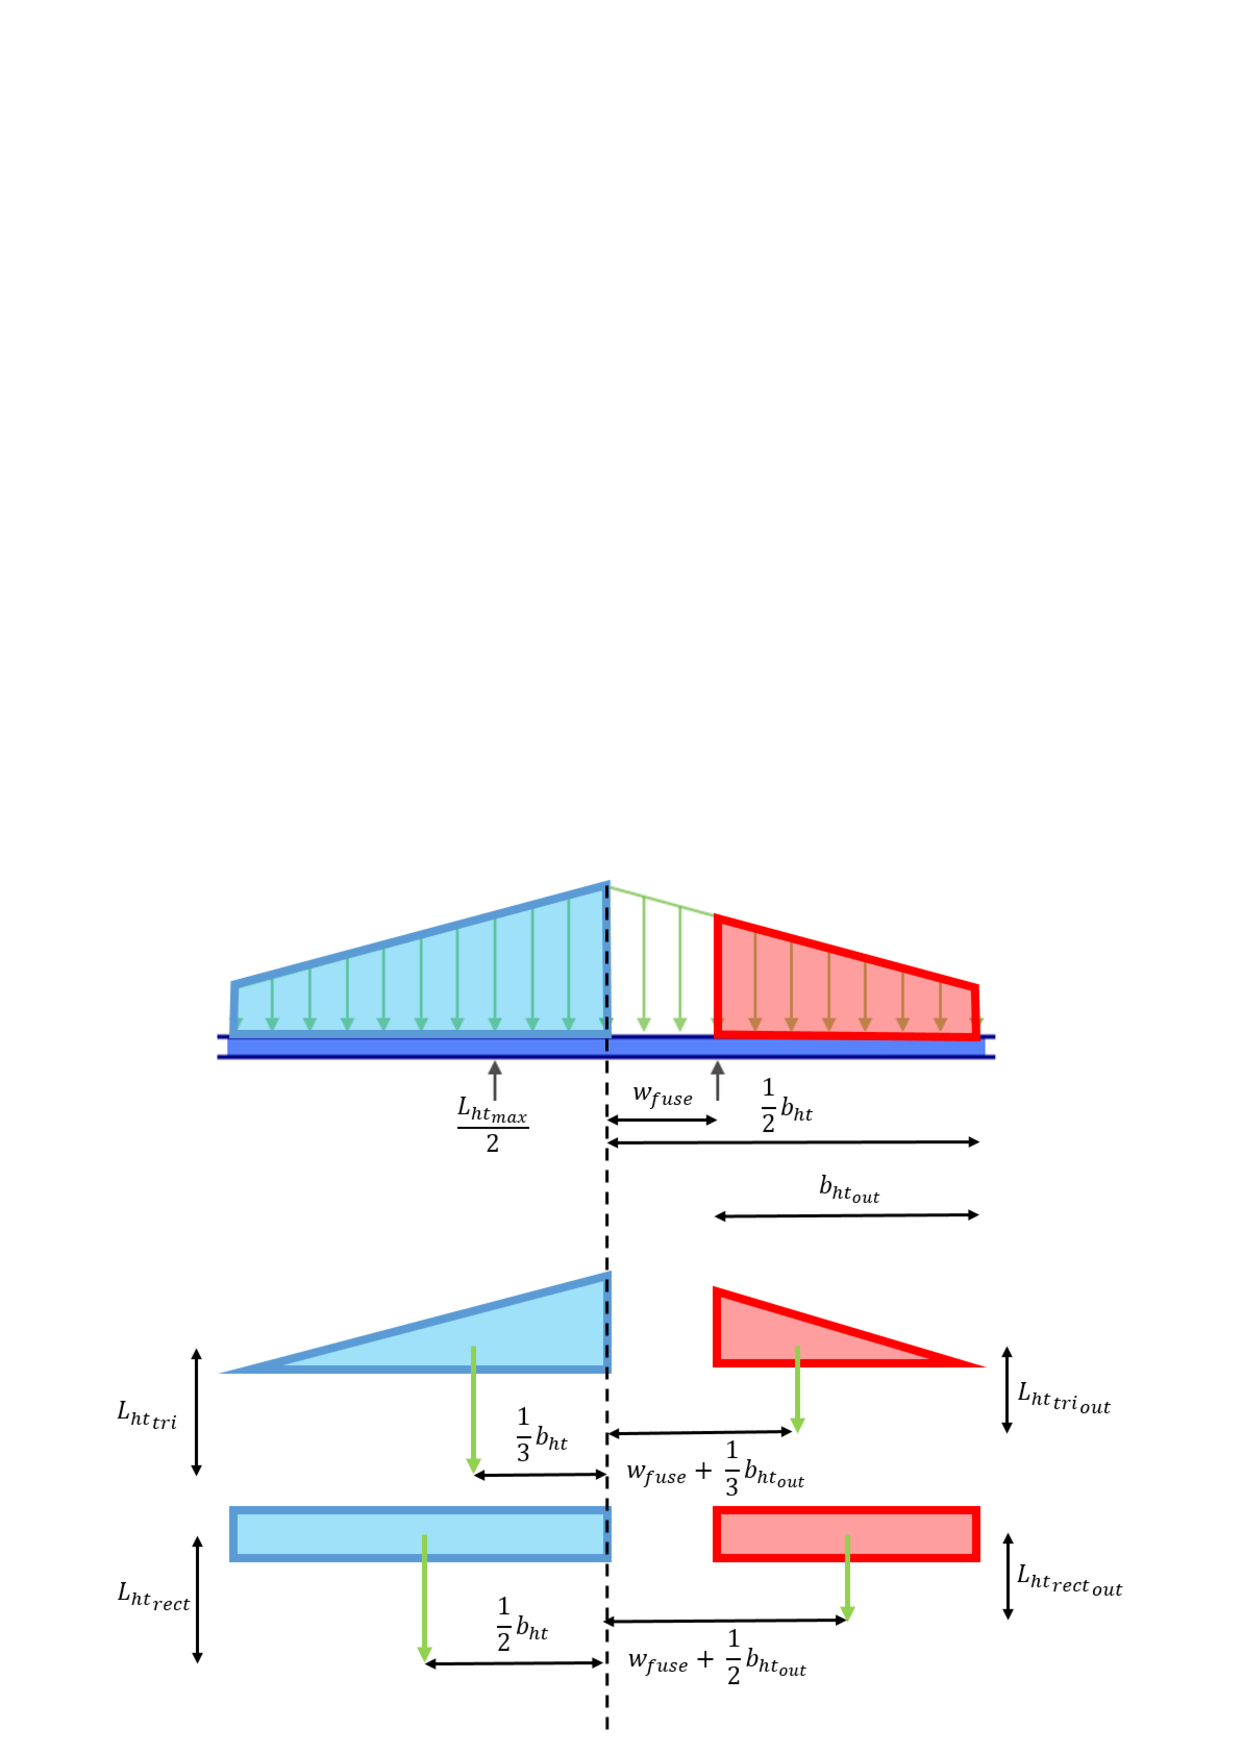
\includegraphics[width=.8\textwidth,natwidth=585,natheight=442]{HTFBD.pdf}
\caption{Free body diagram of the forces on the horizontal tail. The distributed 
lift force, which is assumed to be proportional to local chord, is partitioned 
into triangular and rectangular components.}
\label{fig:HTFBD}
\end{figure}

Shear and moment diagrams are presented in Figures~\ref{fig:HTshear} and 
\ref{fig:HTmoment} respectively. The diagrams include both the distributed lift 
loads (green arrows in Figure \ref{fig:HTFBD}) and the point loads of imposed on 
the pin joints by the vertical tails.

\begin{figure}[!ht]
    \centering
    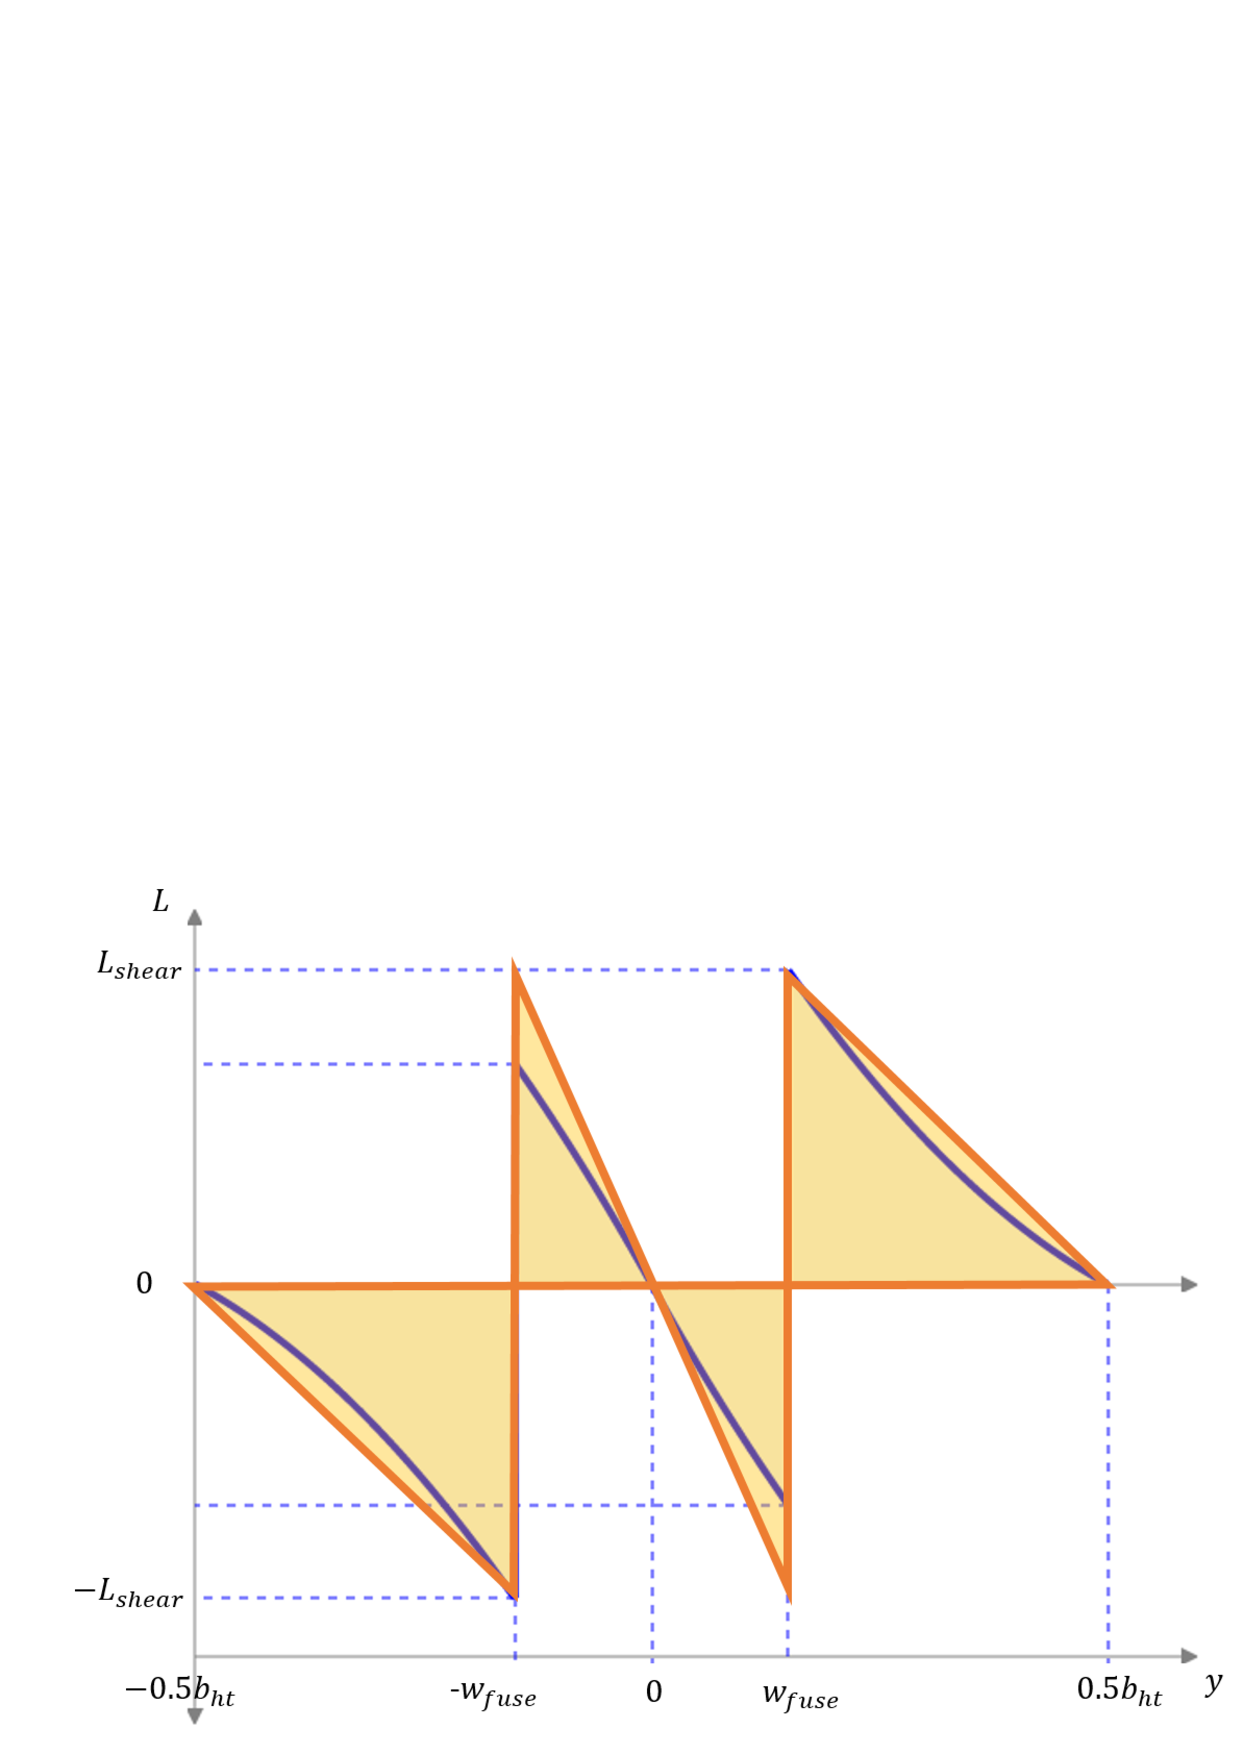
\includegraphics[width = 0.7\linewidth,natwidth=621,natheight=428]{HTshear.pdf}
    \caption{Shear diagram of the pi-tail. The blue line shows the actual 
loading, while the yellow line with infill shows the assumed load distribution.}
    \label{fig:HTshear}
\end{figure}

\begin{figure}[!ht]
    \centering
    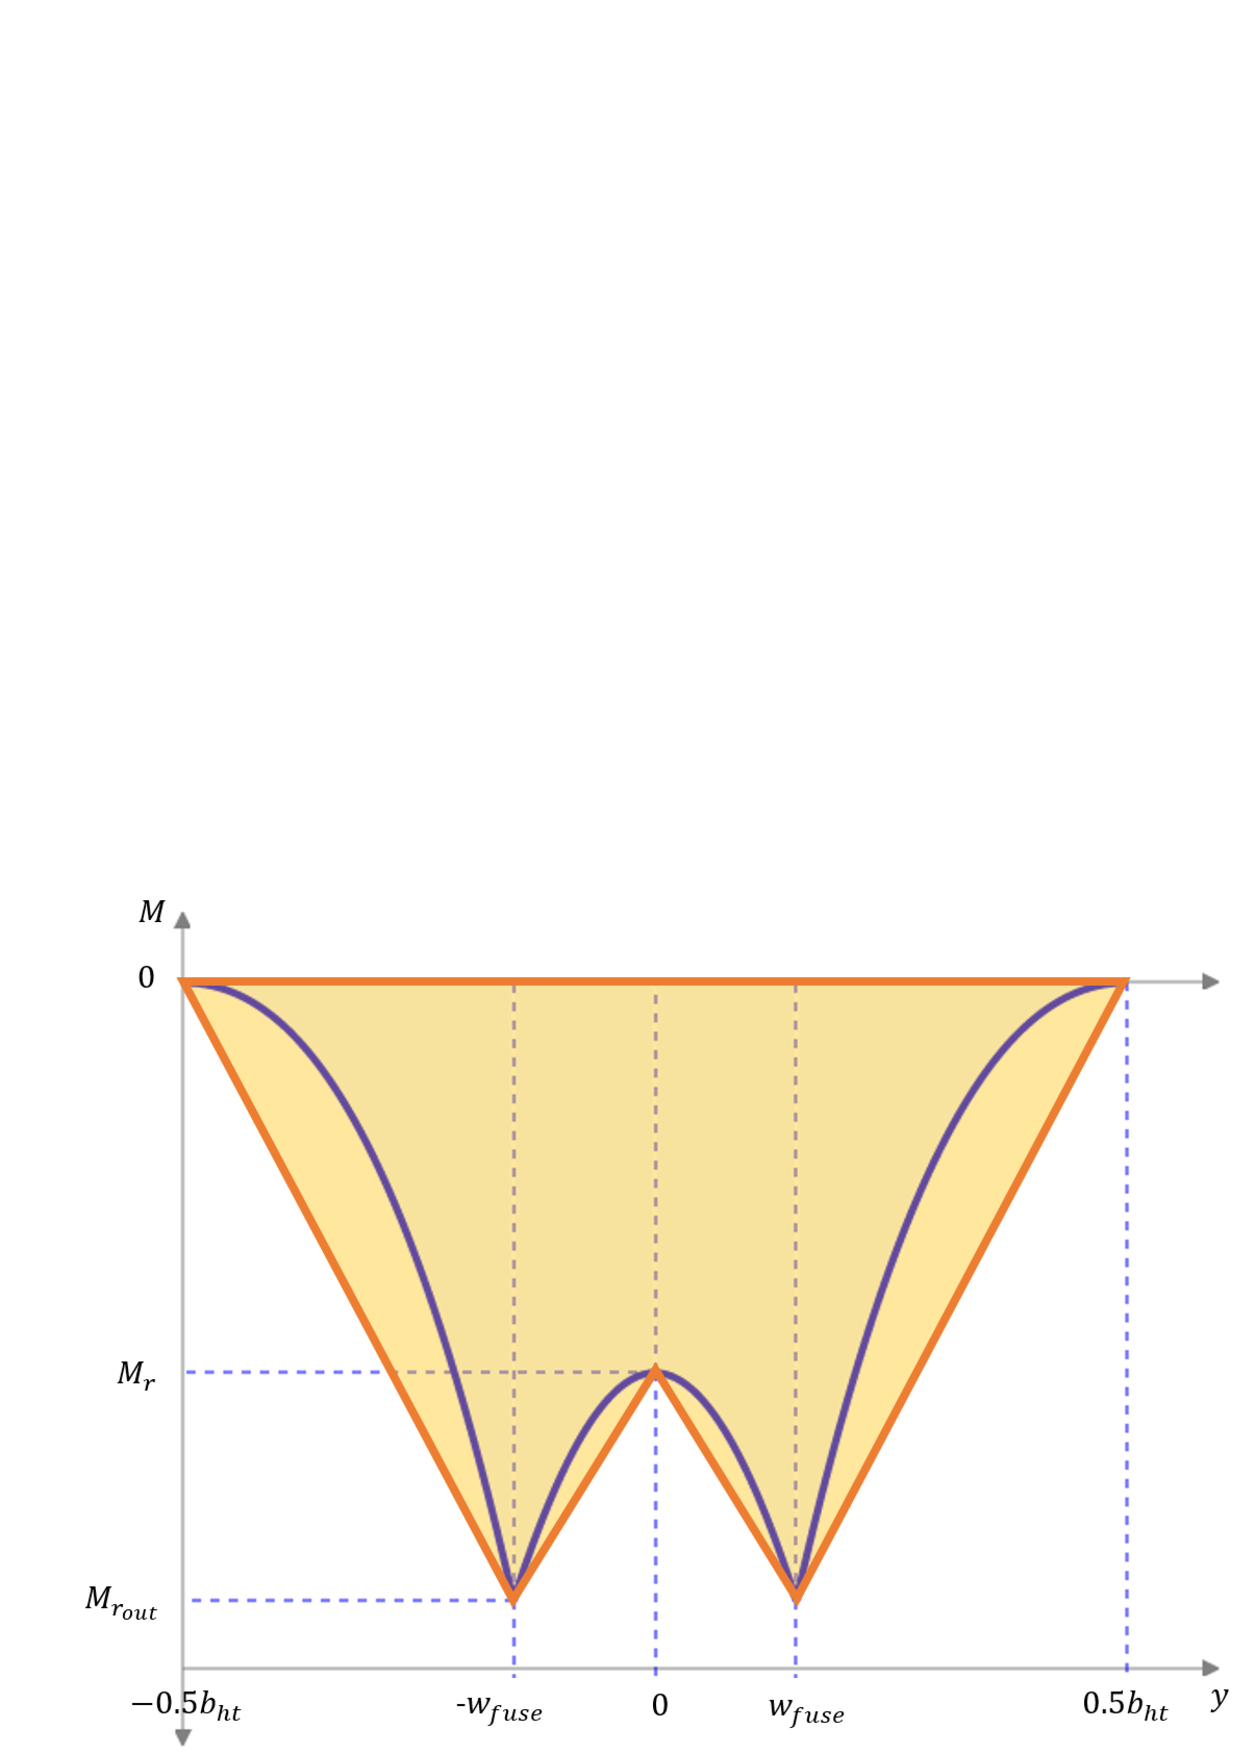
\includegraphics[width = 0.7\linewidth,natwidth=627,natheight=437]{HTmoment.pdf}
    \caption{Moment diagram of the pi-tail. The blue line shows the actual 
loading, and the yellow line shows the assumed load distribution}
    \label{fig:HTmoment}
\end{figure}

After having seen these diagrams, we can make 

The pi horizontal tail becomes a conventional tail in the limit where $w_{fuse} \xrightarrow[]{} 0$. 


After seeing these load distributions, an experienced \gls{GP} modeler would immediately think about linearization. 



The pin-joint assumption ensures the vertical tail structural constraints do not 
need to be modified for the pi-tail configuration. 



\subsubsection{Horizontal Tail Terminology}
\begin{tabbing}
$I_{\rm{cap}}$ = non-dimensional spar cap area moment of inertia \\
$L_{\rm{ht}}$ = horizontal tail downforce \\
$L_{\rm{ht}_{\rm{max}}}$ = maximum horizontal tail downforce \\
$L_{\rm{ht}_{rect}}$ = rectangular horizontal tail load \\
$L_{\rm{ht}_{\rm{rect}_{\rm{out}}}}$ = rectangular horizontal tail load outboard\\
$L_{\rm{ht}_{\rm{tri}}}$ = triangular horizontal tail load \\
$L_{\rm{ht}_{tri_{\rm{out}}}}$ = triangular horizontal tail load outboard\\
$L_{\rm{shear}}$ = maximum shear load at pin-joint\\
$M_{\rm{r}}$ = moment per chord at horizontal tail root \\
$M_{\rm{r}_{\rm{out}}}$ = moment per chord at pin-joint\\
$N_{\rm{lift}}$ = horizontal tail loading multiplier \\
$S_{\rm{ht}}$ = horizontal tail area \\
$W_{\rm{cap}}$ = weight of spar caps \\
$W_{\rm{struct}}$ = horizontal tail wingbox weight \\
$W_{\rm{web}}$ = weight of shear web \\
$\lambda_{\rm{ht}}$ = horizontal tail taper ratio \\
$\nu$ = dummy variable = $(t^2 + t + 1)/(t+1)^2$ \\
$\pi_{\rm{M-fac}}$ = pi-tail bending structural factor \\
$\rho_{\rm{cap}}$ = density of spar cap material \\
$\rho_{\rm{web}}$ = density of shear web material \\
$\sigma_{max,shear}$ = allowable shear stress \\
$\sigma_{\rm{max}}$ = allowable tensile stress \\
$\tau_{\rm{ht}}$ = horizontal tail thickness/chord ratio \\
$b_{\rm{ht}}$ = horizontal tail span \\
$b_{\rm{ht}_{\rm{out}}}$ = horizontal tail outboard half-span\\
$c_{\rm{attach}}$ = horizontal tail chord at the pin-joint \\
$c_{\rm{root}_{\rm{ht}}}$ = horizontal tail root chord \\
$c_{\rm{tip}_{\rm{ht}}}$ = horizontal tail tip chord \\
$g$ = gravitational acceleration \\
$q_{\rm{ht}}$ = substituted variable = 1 + taper \\
$r_h$ = fractional wing thickness at spar web \\
$t_{\rm{cap}}$ = non-dim. spar cap thickness \\
$t_{\rm{web}}$ = non-dim. shear web thickness \\
$w$ = wingbox width-to-chord ratio \\
$w_{\textrm{fuse}}$ = fuselage half-width \\
\end{tabbing}

\subsubsection{Load Derivation}

$L_{\rm{ht}_{rect}}$ is defined to be half the lift generated by the `rectangular' 
section of the wing (the blue rectangle in Figure~\ref{fig:HTFBD}).

\begin{equation}
    L_{\rm{ht}_{rect}} \geq \frac{L_{\rm{ht}_{\rm{max}}} c_{\rm{tip}_{\rm{ht}}} b_{\rm{ht}}}{2 S_{\rm{ht}}}
\end{equation}

Similarly, $L_{\rm{ht}_{\rm{tri}}}$ is defined to be half the lift generated by the 
`triangular' section of the wing (the blue triangle in Figure~\ref{fig:HTFBD}).
 
\begin{equation}
     L_{\rm{ht}_{\rm{\rm{tri}}}} \geq \frac{L_{\rm{ht}_{\rm{max}}} (1 - \lambda_{\rm{ht}}) c_{\rm{root}_{\rm{ht}}} b_{\rm{ht}}}{4 
S_{\rm{ht}}}
\end{equation}
 
After defining the horizontal tail half-span outboard of the pin joint 
($b_{\rm{ht}_{\rm{out}}}$), the outboard components of the lift loads   can be computed 
with respect to $L_{\rm{ht}_{rect}}$ and $L_{\rm{ht}_{\rm{tri}}}$. The outboard loads are shown 
in red in Figure~\ref{fig:HTFBD}. 
 
 \begin{align}
     b_{\rm{ht}_{\rm{out}}} &\geq 0.5b_{\rm{ht}} - w_{\textrm{fuse}}\\
     L_{\rm{ht}_{tri_{\rm{out}}}} &\geq L_{\rm{ht}_{\rm{tri}}} \frac{b_{\rm{ht}_{\rm{out}}}}{(0.5b_{\rm{ht}})^2}\\
     L_{\rm{ht}_{\rm{rect}_{\rm{out}}}} &\geq L_{\rm{ht}_{rect}} \frac{b_{\rm{ht}_{\rm{out}}}}{0.5b_{\rm{ht}}}
 \end{align}
 
The horizontal-vertical tail pin joint is assumed to be exactly at $w_{\textrm{fuse}}$. 
This is a conservative estimate. In most pi-tail configurations the vertical 
tails are canted outwards. The local chord at the pin joint is constrained with 
the following monomial equality.
 
\begin{equation}
    c_{\rm{attach}} = \frac{b_{\rm{ht}} \lambda_{\rm{ht}} c_{\rm{root}_{\rm{ht}}}}{2 w_{\textrm{fuse}}}
\end{equation}
 
The maximum moment at the joint is determined by summing the bending moment 
contributions from loads outboard of the joint. 
\begin{equation}
M_{\rm{r}_{\rm{out}}} c_{\rm{attach}} \geq 
                    L_{\rm{ht}_{\rm{rect}_{\rm{out}}}} \frac{1}{2}b_{\rm{ht}_{\rm{out}}} + 
L_{\rm{ht}_{tri_{\rm{out}}}} \frac{1}{3}b_{\rm{ht}_{\rm{out}}},
\end{equation}
 
The maximum shear at the joint is the sum of the outboard shear loads. The 
maximum root moment is the sum of the bending loads from lift and the pin-joint 
load. 
 
\begin{align}
L_{\rm{shear}} &\geq L_{\rm{ht}_{\rm{rect}_{\rm{out}}}} + L_{\rm{ht}_{tri{\rm{out}}}}\\
M_{\rm{r}} c_{\rm{root}_{\rm{ht}}} &\geq L_{\rm{ht}_{\rm{rect}}} \frac{1}{4}b_{\rm{ht}} + L_{\rm{ht}_{\rm{\rm{tri}}}} 
\frac{1}{6}b_{\rm{ht}}  - \frac{1}{2}L_{\rm{ht}_{\rm{max}}} w_{\textrm{fuse}} 
\end{align}

Finally, the wingtip moment is set equal to zero with a signomial equality 
constraint.

\begin{equation}
    \frac{b_{\rm{ht}}}{4} L_{\rm{ht}_{\rm{rect}}} + \frac{b_{\rm{ht}}}{3} L_{\rm{ht}_{\rm{\rm{tri}}}} = b_{\rm{ht}_{\rm{out}}} 
\frac{L_{\rm{ht}_{\rm{max}}}}{2}
\end{equation}

\subsubsection{Structural Sizing}

Equations from \cite{gp_ac_design} for wing structural sizing were adapted using 
a linearization of the moment and shear load distributions from Appendix E2. The 
constraints can be applied to both conventional and pi-tails.

\begin{align}
    0.92 w\tau_{\rm{ht}} t_{\rm{cap}}^2 + I_{\rm{cap}} &\leq \frac{0.92^2}{2}w\tau_{\rm{ht}}^2t_{\rm{cap}}\\
    8 &\geq N_{\rm{lift}}M_{\rm{r}_{\rm{out}}}(\AR_{\rm{ht}})q_{\rm{ht}}^2\frac{\tau_{\rm{ht}}}{S_{\rm{ht}} I_{\rm{cap}}\sigma_{\rm{max}}}\\
    12 &\geq \frac{2L_{\rm{shear}} N_{\rm{lift}} q^2}{\tau_{\rm{ht}} S t_{\rm{web}} \sigma_{\rm{max-shear}}}
\end{align}

The changes to the model in \cite{gp_ac_design} are:
\begin{itemize}
    \item In the shear constraint replacing $L_{\rm{ht}_{\rm{max}}}$ with $2L_{\rm{shear}}$. 
This is done because the shear loads for the pi-tail are different than the 
maximum lift loads for the conventional tail. 
    \item Replacing $M_{\rm{r}}$ with $M_{\rm{r}_{\rm{out}}}$, the moment per unit chord at the 
pin joint. For a pi-tail, maximum bending loads occur at the pin joint.
    %, and along with the root moment per unit chord $M_{\rm{r}}$ can be used to give a 
    %conservative approximation for the mass of the horizontal tail. 
\end{itemize}

The linearization of the shear and bending load distributions simplifies the 
derivation of the structural web and cap weights. Shear web sizing relies on the 
assumption that the maximum shear ($L_{\rm{shear}}$) occurs at the pin-joint and the 
weight of the shear web of the pi-tail under $L_{\rm{shear}}$ is equal to the shear 
web weight of a conventional tail subjected to the the same maximum shear load 
at its root. This is a conservative approximation, the load distribution implied 
by this assumption (shown in yellow in Figure~\ref{fig:HTshear}) has a larger 
internal area than the actual load distribution. Intuitively, the $L_{\rm{shear}}$ 
for a pi-tail is strictly smaller than the $L_{\rm{shear}}$ a conventional tail of 
the same size and loading. The pi-tail more efficient in shear.

The cap weight of the pi-tail is determined by scaling the cap weight of a 
conventional tail with the same geometry as the pi-tail and a root moment of 
$M_{\rm{r}_{\rm{out}}} c_{\rm{attach}}$. The scaling factor, $\pi_{\rm{M-fac}}$, is the ratio of the 
total shaded bending moment area in Figure~\ref{fig:HTmoment} to the sum of the 
outboard shaded areas multiplied by the ratio of the outboard half-span to the 
total half-span.

\begin{equation}
    \pi_{\rm{M-fac}} \geq \left[\frac{\frac{1}{2}(M_{\rm{r}_{\rm{out}}} c_{\rm{attach}} +
    M_{\rm{r}} c_{\rm{root}_{\rm{ht}}}) w_{\textrm{fuse}}} {\frac{1}{2}M_{\rm{r}_{\rm{out}}} c_{\rm{attach}} 
b_{\rm{ht}_{\rm{out}}}} + 1.0\right]
    \frac{b_{\rm{ht}_{\rm{out}}}} {0.5b_{\rm{ht}}},
\end{equation}

Given the calculated loads and structural factors, the bending material and 
shear web weight can be calculated. 

\begin{align}
    W_{\rm{cap}} &\geq \frac{\pi_{\rm{M-fac}} 8 \rho_{\rm{cap}} g w t_{\rm{cap}} S_{\rm{ht}}^1.5 \nu}
    {3\AR_{\rm{ht}}^{0.5}}\\
    W_{\rm{web}} &\geq \frac{8 \rho_{\rm{web}} g r_h \tau_{\rm{ht}} t_{\rm{web}} S_{\rm{ht}}^{1.5} 
\nu}{3\AR_{\rm{ht}}^{0.5}}\\
    W_{\rm{struct}} &\geq W_{\rm{web}} + W_{\rm{cap}}
\end{align}

The value for $t_{\rm{cap}}$ is notional in the derivation above. Rather than being 
the spar cap thickness of a pi-tail, it is the spar cap thickness required for a 
conventional tail of the same geometry and a root moment  ($M_{\rm{r}_{\rm{out}}} 
c_{\rm{attach}}$) as a pi-tail. With a similar reasoning as for the shear loads, 
$\pi_{\rm{M-fac}} t_{\rm{cap}}$ for a pi-tail is strictly smaller than the $t_{\rm{cap}}$ for a 
conventional tail of the same geometry and loading, making the pi-tail more 
efficient in bending than a traditional tail. 

\subsection{Further potential horizontal tail model extensions}
\label{sec:HTExtensions}
\appendix
%\include{appa}
%\include{appb}
\include{biblio}
\end{document}

